\chapter{Machinelles Lernen}

Der Themenbereich des \keyword{Machinellen Lernens} beschäftigt sich mit Algorithmen und mathematischen Modellen, welche von selber lernen, Probleme zu loesen.
Hierbei wird nicht explizit einprogrammiert, wie das Modell das Problem zu loesen
hat, stattdessen wird das Modell trainiert, optimiert sich von selbst und findet selber
einen Weg, das Problem zu loesen.
Die Grundidee dabei ist, dass man Daten erfasst, generiert oder misst, welche
analysiert werden sollen. Innerhalb dieser Daten existieren gewisse
Gesetzmaessigkeiten und Mustern. Diese Muster sollen vom Modell
erkannt werden und verallgemeinert werden. Nach dem erfolgreichen Lernen,
kann das Modell Vorhersagen zu neuen Daten machen.
\para{}
Man unterscheiden zwischen zwei Arten von Maschinellen Lernen.
\begin{itemize}
\item{
    \keyword{Ueberwachtes Lernen} (engl.:\ supervised learning) ist ein
    Lernverfahren, bei welchem die Daten aus zwei Teilen bestehen, aus Inputs und
    Outputs. Man bezeichnet dabei die Outputs als Labels. Die Aufgabe des Modells
    ist es eine \keyword{Korrelation} zwischen den Inputs und den Labels zu
    erlernen und so ihre Beziehung zueinander zu verstehen.
    Anhand der Informationen, welche in den Inputs enthalten
    sind, sind dann die Labels vorherzusagen. Man gleicht dann die
    vorhergesagten Labels des Modells mit den wahren Labels ab (man ``ueberwacht'' sie) und bewertet so ihre Faehigkeiten.
    \para{}
    Voraussetztung dafuer ist, dass die Daten eben ``gelabelt'' sein muessen.
    Man muss schon im vorhinein Daten haben, bei welchen man die gewuenschten
    Labels hat. Natuerlich muss auch die erwaehnte Korrelation bestehen. Falls
    kein Zusammenhang zwischen den Inputs und den Outputs besteht, kann das
    Modell auch keine Vorhersagen machen und so auch nichts erlernen.
  }
\item{
    \keyword{Unueberwachtes Lernen} (engl.:\ unsupervised learning) ist ein anderes
    Lernverfahren, bei welchem eben diese Labels nicht vorhanden sind. Dem
    Modell stehen nur die Inputdaten zur Verfuegung. Diese werden auch analysiert
    und das Modell soll Muster herausextrahieren, welche sich von sonstigem
    zuefaelligen Rauschen unterscheiden.
  }
\end{itemize}

Der Grossteil der Modelle des Maschinellen Lernens benutzten ueberwachtes
Lernen, da es auch deutlich mehr Anwendungsmoeglichkeiten besitzt. Es gibt nur wenige Arten von
unueberwachtem Lernen, dazu gehoeren: Hauptkomponentenanalysen und Generative
Adversial Networks. Aus diesem Grund, werden wir im folgenden uns grundsaetzlich
mit ueberwachtem Lernen beschaeftigen.
\para{}
\cite{wiki:supervised_learning}
\cite{wiki:unsupervised_learning}

\section{Allgemeine Begriffe}

\subsection{Korrelation?}

\subsection{Daten}

Um ein Modell zu trainieren braucht man Daten. Diese Daten bestehen immer aus
\keyword{Inputs} und aus \keyword{Outputs}. Man unterscheidet hierbei zwei Arten
von Outputs. Die \keyword{Labels} sind die erwarteten Outputs, welche die
gewueschten Zielwerte sind. Die \keyword{Vorhersagen} sind die Outputs, welche
das Modell produziert und hoffentlich moeglichst genau mit den Labels
uebereinstimmen.
\para{}
Diese Daten fuer Training kommen in der Form eines \keyword{Trainingsdatensatz} $\set{X}$.
Dabei handelt es sich um eine Menge von \keyword{Samples},
welche jeweils aus Inputs und Labels bestehen.
Die Inputs werden in einem Vektor
\[ \vec{x} = \trans{\begin{pmatrix} x_1 & x_2 & \cdots & x_m \end{pmatrix}} \]
und die Labels in einem Vektor
\[ \vec{\hat{y}} = \trans{\begin{pmatrix} \hat{y}_1 & \hat{y_2} & \cdots & \hat{y}_n \end{pmatrix}} \]
zusammengefasst. Auch die Vorhersagen werden in einem Vektor
\[\vec{y} = \trans{\begin{pmatrix} y_1 \quad y_2 \quad \cdots \quad y_n \end{pmatrix}} \]
zusammengefasst.
Somit ist ein Trainingssample nichts anderes als ein Paar
$(\vec{x}_i,\vec{\hat{y}}_i)$ eines Inputsvektor $\vec{x}$ und eines Labelvektor
$\vec{\hat{y}}$.
\para{}
Die Inputs bestehen aus gewissen \keyword{Attributen}, welche die
Merkmals\textit{typen} der Daten sind. Die sogennanten \keyword{Features} sind
dann die spezifischen Werte der Attribute eines Samples. Der Algorithmus soll
anhand dieser Features seine Vorhersagen machen.
Diese Vorhersagen werden dann mit den Labels abgeglichen und so bewertet.
Anhand der Bewertungen wird dann eine Optimierung des Modells vorgenommen.
Unter korrekten Bedingungen (kein Overfitting) findet kein Auswendiglernen der Trainingsdaten statt,
sondern ein Generalisieren des Zusammenhangs anhand von Mustern und Gesetzmassigkeiten.
\para{}
Um eine endgueltige Bewertung des Modells durchzufuehren, wird ein Testdatensatz
$\set{T}$, welcher nicht Teil des Trainingsdatensatz ist, genutzt um Vorhersagen zu machen.
Dies garantiert, dass kein Auswendiglernen moeglich ist.
\para{}
BEISPIEL


\subsection{Modelle}
Ein \keyword{Modell} ist eine mathematische Funktion $\mathit{h}\colon \set{R}^m
\to \set{R}^n$, Hypothesenfunktion gennant, welche die Inputs auf die Outputs abbildet $\vec{y}=\mathit{h}(\vec{x})$.
Man kann diese Funktion gewissermassen als die Hypothese, welche das Modell bezueglich der Beziehung zwischen
den Inputs und den Labels aufgestellt hat, betrachten.
Diese Modelle koennen verwendet werden um vorallem entweder
Klassifizierungsprobleme oder Regressionsprobleme zu loesen. Falls es sich um
letzteres handelt, spricht man von einem Regressionsmodell. Ein solches
Regressionsproblem werden wir in dieser Arbeit loesen.
\para{}
Das Verhalten eines Modells wird bestimmt durch seine \keyword{Modellparameter}
$\param_1, \param_2,\ldots,\param_k$. Sie bestimmen, wie die Hypothese des Modells lautet.
Das Ziel ist es, die Modellparameter so einzustellen, dass die Vorhersagen
$\vec{y}$ des Modells besser mit den Labels $\vec{\hat{y}}$ der Trainingsdaten uebereinstimmen.
Dies wird iterativ gemacht, indem immer wieder leichte Anpassungen an den
Parametern vorgenommen werden, bis das Modell die gewuenschten Resultate liefert.
\para{}
Neben den gelernten Parametern, gibt es auch noch sogenannte \keyword{Hyperparameter}.
Diese koennen nicht erlernt werden, sondern muessen manuell vor dem Training gewaehlt werden und koennen den Lernvorgang erheblich beeinflussen.
Dies bedeutet, dass man ausprobieren muss, welche Werte fuer die Hyperparameter
die besten Resultate liefern.
\para{}
Das wohl einfachste Regressionsmodell ist eine Regressionsgerade. Diese ist
angemessen, falls ein einfacher linearen Zusammenhang der Form $y=\param_1x +
\param_0$ zwischen den Features und den Labels besteht.
Nun muessten nur noch $\param_0$ und $\param_1$ bestimmt werden.
BEISPIELMODELL AUTO
\para{}
Fuer Machine Learning haben sich gewisse Modelle besonders guet etabliert,
darunter waeren: Support Vector Machines, Evolutionäre Algorithmen, und Künstliche Neuronale Netze.
Diese Arbeit wird sich vorwiegend mit Neuronalen Netzen auseinandersetzen.
\\
\begin{figure}[h!]
  \centering


  \caption{Schema eines Modells}
\end{figure}

\section{Training}
\subsection{Verlust- und Kostenfunktionen}
Einsicht ist der erste Schritt zur Besserung. Das gilt auch beim Machine Learning, deshalb muss beim Training zuerst die Genauigkeit des Modells bewertet werden.
Dies wird mithilfe von sogennaten Kostenfunktion bzw. Verlustfunktionen
erreicht.
\para{}
Eine \keyword{Verlustfunktion} $L(y,\hat{y})$ sollte ein Mass fuer die
Abweichung der Vorhersagen $y$ von den Labeln $\hat{y}$ sein.
Aus ihr bildet man die \keyword{Kostenfunktion} $C(\vec{y},\vec{\hat{y}})$, indem man die
alle Verluste der einzelnen Ouputs aufsummiert. Somit erhaelt man die Kosten
einer gesamten Vorhersage mit $m$ Outputs (siehe Gl. (\ref{eq:errorfunc})). \\
Der Fehler $\bar{C}(\set{X})$ des gesamten Trainingsdatensatz $\set{X}$, der
Groesse $p$, ergibt sich aus dem arithemtischen Mittel der einzelnen Kosten der
Vorhersagen (siehe Gl. (\ref{eq:meanerrorfunc})).
\\
\begin{minipage}[h!]{0.5\textwidth}
  \begin{equation}\label{eq:errorfunc}
    C \left(\vec{y},\vec{\hat{y}} \right) = \ds\sum_{i=1}^{m} L(y_i, \hat{y}_i)
  \end{equation}
\end{minipage}
\begin{minipage}[h!]{0.5\textwidth}
  \begin{equation}\label{eq:meanerrorfunc}
    \bar{C}(\set{X}) = \frac{1}{p}\ds\sum_{j=1}^{p} C\left(\vec{y}_j,\vec{\hat{y}}_j\right)
  \end{equation}
\end{minipage}
\para{}
Eine Verlustfunktion $L$ bzw. eine Kostenfunktion $C$ sollte folgende Eigenschaften aufweisen:
\begin{itemize}
\item{$L$ ist minimal, wenn $y = \hat{y}$}
\item{$L$ waechst mit $|y - \hat{y}}|$}
\item{$C$ ist nach jedem $y_n$ partiell differenzierbar (erklaert in Sektion (\ref{ref:partielle_ableitungen}))}
\end{itemize}
\para{}

\subsubsection{Mittlere quadratische Abweichung}
Die bekannteste Verlustfunktion ist die ``Mittlere quadratische Abweichung''
(engl.:\ mean squared error). Sie ist definiert als das arithmetische Mittel
aller quadrierten Differenzen zwischen den Vorhersagen und Labels.
Zusaetzlich halbiert man noch das arithmetische Mittel, damit bei der Ableitung der Faktor
$2$ wegfaellt.
\\
\begin{equation}\label{eq:MSE}
  L_{MSE} = \frac{1}{2n}{(\hat{y} - y)}^2
\end{equation}
\\
Die Kostenfunktion kann mithilfe des einer Summe berechnen werden, oder in
diesem Fall mithilfe einer Vektorsubtraktion Vorhersagen $\vec{y}$ von den Labels $\vec{\hat{y}}$.
\\
\begin{equation}\label{eq:MSE}
  C_{MSE} = \frac{1}{2n}\sum_{i=1}^{n}{(\hat{y}_i - y_i)}^2 = \frac{1}{2n}{(\vec{\hat{y}} - \vec{y})}^2
\end{equation}
\\
Sie erfuellt alle Anforderungen an eine Kostenfunktion:
\begin{itemize}
\item{Ihr Funktionwert ist 0 und minimal fuer $\vec{y} = \vec{\hat{y}}$}
\item{Sie ist proportional zu ${(\vec{\hat{y}}-\vec{y})}^2$}
\item{Ihre partielle Ableitung nach einem $y_i$ lautet: $C_{MSE}'=\frac{1}{n}(y_i-\hat{y_i})$}
\end{itemize}


\subsubsection{Cross-entropy}


\subsection{Gradientenverfahren}\label{sec:gradientenverfahren}
Um ein Modell nun zu trainieren, muss man verstehen, dass es sich um ein Optimierungsproblem handelt.
Das Modell ist am besten, also macht die besten Vorraussagen, wenn die
Funktionswerte der Kostenfunktion am kleinsten sind.
Deshalb muss diese Kostenfunktion $C$ minimiert werden.
Hierbei muss die Funktion $C$ nicht mehr in Abhaengigkeit der Inputs betrachtet
werden, sondern als Funktion der Modellparametern
$C(\param_1, \param_2, \ldots, \param_k)$, denn diese sollen angepasst werden,
um das Modell zu verbessern. $\ds (\param_1,\ldots,\param_k) = \operatorname*{\arg
  \min}(C)$.
Fuer diese Optimiertung wird das sogennante \keyword{Gradientenverfahren} (engl.: Gradient descent) verwendet.
\footnote{
  Im Gymnasium wird beigebracht die lokalen Extrema (inkl.\ lokalen Minimas) zu bestimmen, indem die erste Ableitung $f'$ gebildet wird und  gleich null gesetzt wird.
  Dies ist hier nicht moeglich, da die Funktion $C'(\param_1,\param_2, \ldots,
  \param_n)$ deutlich zu komplex ist, um die Nullstellen analytisch zu bestimmen. Deshalb wird das Gradientenverfahren verwendet.
}
\para{}
Allgemein koennen mithilfe des Gradientenverfahrens Funkionen $f(x_1, x_2, \ldots, x_n)$ vom Typ $\set{R}^n \to \set{R}$ (wie z.B. die Fehlerfunktion) minimiert werden.
Dies geschieht, indem ein Startpunkt (Ortsvektor) $\vec{p}_0$, dessen
Komponenten den Input von $f(\vec{p}_0)$ darstellt, gewaehlt wird.
Nun werden iterativ neue Punkte $\vec{p}_t$ gesucht, welche immer naeher beim lokalen Minimun liegen, also Punkte, die den Funktionswert $f(\vec{p}_t)$ immer kleiner werden lassen.
Dies wird durchgeführt, bis der Punkt genug nahe beim lokalen Minimun ist.
\para{}
Dafuer muss ein Vektor $\vec{b}_t$ bestimmt werden, welcher auf den Punkt $\vec{p}_t$ draufaddiert einen neuen Punkt $\vec{p}_{t+1}$ bildet,
bei dem der Funktionswert $f(\vec{p}_{t+1})$ kleiner ist als der von $f(\vec{p}_t)$.
Dies geschieht am effizientesten, wenn $\vec{b}_t$ in die Richtung der staerksten Funktionswertabnahme zeigt.

Hierzu braucht man den sogennanten \keyword{Gradient} $\vecf{\nabla}$, wofür man wiederum partielle Ableitungen braucht.
\para{}
\begin{defbox}{Partielle Ableitungen}\label{ref:partielle_ableitungen}
  Partielle Ableitungen sind eine Erweiterung der ``normalen'' Ableitungen auf
  multidimensionale Funktionen $f(\vec{x}) = f(x_1,\ldots,x_n): \set{R}^n \to \set{R}$.
  Man leitet dabei nur nach einem Argument $x_i$ ab und betrachtet die restlichen Argumente als Konstanten.
  Es gelten die gleichen Ableitungsregeln wie bei der nicht-partiellen Ableitung.
  Die partielle Ableitung einer Funktion $f(x_1,\ldots,x_n)$ bezueglich einer
  Variable $x_i$ in einem Punkt $\vec{a} = \trans{\begin{pmatrix} a_1 & \cdots & a_n \end{pmatrix}}$
  ist analog zur normalen Ableitung folgendermassen definiert:
  \begin{equation*}
    \partderiv{f}{x_i}(\vec{a}) \coloneqq \lim_{h \to 0} \frac{f(a_1,\ldots,a_i + h,\ldots,a_n)-f(a_1,\ldots,a_i,\ldots,a_n)}{h}
  \end{equation*}
  Geometisch ist dies die Steigung der Tangente an die Funktion $f$ im Punkt
  $\vec{a}$. Die Tangente liegt in der Richtung der Achse des Parametern $x_i$, nach dem man ableitet.
\end{defbox}
\\
\begin{defbox}{Gradient}
  Der Gradient $\vecf{\nabla}$ ist ein Differentialoperator, den man auf eine
  Funktion $f(\vec{x}) = f(x_1,\ldots,x_n): \set{R}^n \to \set{R}$ anwendet kann, welcher ein Skalarfeld auf ein Vektorfeld (das sogennante Gradientenfeld) abbildet.\\
  Um den Gradienten $\vecf{\nabla}f$ der Funktion $f$ zu bilden, fasst man alle partiellen Ableitungen der Funktion $f$, nach jedem
  Argument $x_i$, in einem Vektor zusammen. Meistens bestimmt man den Gradienten
  $\vecf{\nabla} f(\vec{p})$ in einem spezifischen Punkt $\vec{p} =
  \trans{\begin{pmatrix} p_1 & \cdots & p_n \end{pmatrix}}$.
  \begin{equation*}
    \vecf{\nabla}_{\vec{x}} f(\vec{p}) = \ds\partderiv{f}{\vec{x}}(\vec{p}) =
    \begin{pmatrix}
      \ds\partderiv{f}{x_1}(\vec{p}) \\
      \vdots \\
      \ds\partderiv{f}{x_n}(\vec{p}) \\
    \end{pmatrix}
  \end{equation*}

  Geometisch ist der Gradient $\vecf{\nabla}f(\vec{p})$ einer Funktion $f$ in einem Punkt $\vec{p}$ dann der Vektor, welcher in die Richtung des steilsten Anstiegs von $f$ zeigt.
  Sein Betrag gibt die Staerke des Anstiegs an.

  MATRIX-GRADIENT EINBRINGEN
\end{defbox}
\para{}
\begin{figure}[h!]
  \caption{Skalarfeld mit zugehoerigem Gradientenfeld}
\end{figure}

Da der Gradient in die Richtung des steilsten Anstiegs zeigt, sollte der Vektor
$\vec{b}_t$ gerade in die entgegengesetze Richtung zeigen. Also sollte er in die Richtung des negierten Gradient der Funktion $f$ im Punkt $\vec{p}_t$ zeigen.
Also kann jetzt das iterative Annahern an das lokalen Minimums folgendermassen beschrieben
werden (wobei $\eta$ eine spaeter erklaerte Schrittgroesse darstellt).
\\
\begin{equation}\label{eq:gradientdescent}
  \vec{p}_{t+1} = \vec{p}_t - \eta \cdot \vecf{\nabla} \mathit{f}(\vec{p}_t)
\end{equation}
\\

\ifcp
\begin{figure}[h!]
  \centering
  \begin{tikzpicture}
    \begin{axis}[
      % hide axis,
      xticklabels={,,},
      yticklabels={,,},
      zticklabels={,,},
      xlabel=$x_1$,
      ylabel=$x_2$,
      colormap/cool,
      legend style={at={(1,1.2)},anchor=north east},
      reverse legend
      ]
      \addplot3[domain=-1:1,orange, quiver={u={(1+exp(-(x^2+y^2)))^(-2)*exp(-(x^2+y^2))*(-2*x)}, v={(1+exp(-(x^2+y^2)))^(-2)*exp(-(x^2+y^2))*(-2*y)}, scale arrows=0.4}, -stealth,samples=10] {0.5};
      \addlegendentry{$-\vecf{\nabla}_{\vec{x}}f$}

      \addplot3[
      mesh,
      samples=50,
      domain=-1:1,
      ]
      {1/(1+exp(-(x^2+y^2)))};
      \addlegendentry{$f(x_1,x_2)$}

      \coordinate (ballpos) at (axis cs:-0.8,0.8,{1/(1+exp(-((-0.8)^2+(0.8)^2)))});
      \coordinate (bottom) at (axis cs:0,0,0.5);
      \draw[red,very thick,->,>=latex] (ballpos) -- ($(ballpos)!0.3!(bottom)$);
      \shade [ball color=yellow] (ballpos) circle (0.25cm);
    \end{axis}
  \end{tikzpicture}
  \caption{Visualisierung des Gradientenabstiegs: ein Ball rollt das
    Gradientenfeld hinab in das lokale Minimum.}
\end{figure}
\fi

Waehrend des Gradientenverfahren konvergiert der Punkt $\vec{p}_t$ zu einem
beliebigen \textit{lokalen} Minimum, abhängig davon wie der Startpunkt
$\vec{p}_0$ gewaehlt wurde.
Wie man diesen Startpunkt zu waehlen hat, wird in Sektion
(\ref{sec:parameter_initalisieren}) erlauetert.
Da dieser meist zufaellig bestimmt wird, ist es eine Glückssache ein sehr niedriges Minimum zu finden.
\para{}
Die sogennante \keyword{Lernrate} $\eta$ aus Gleichung (\ref{eq:gradientdescent}) ist ein Hyperparameter.
Sie ist ein positiver Proportionalitatsfaktor, welcher die Schrittgroesse des Gradientenabstieg bestimmt. Sie muss je nach zu minimierender Funktion anderst gewaehlt werden.
Dabei hilft nur ausporbieren. Falls $\eta$ nicht gut gewahelt wurde, gibt es Probleme beim Training:
\begin{itemize}
\item{Falls $\eta$ zu klein ist, verlaueft das Trainings unnoetig langsam und braucht sehr lange.
    Ausserdem kann es passieren, dass man bei einem hohen lokalen Minimum stecken bleibt.}

\item{Falls $\eta$ zu gross ist, kann es passiert, dass man ueber das lokale
    Minimum hinaus schiesst und somit nur darum herum springt.}
\end{itemize}

\begin{figure}[h!]
  \centering
  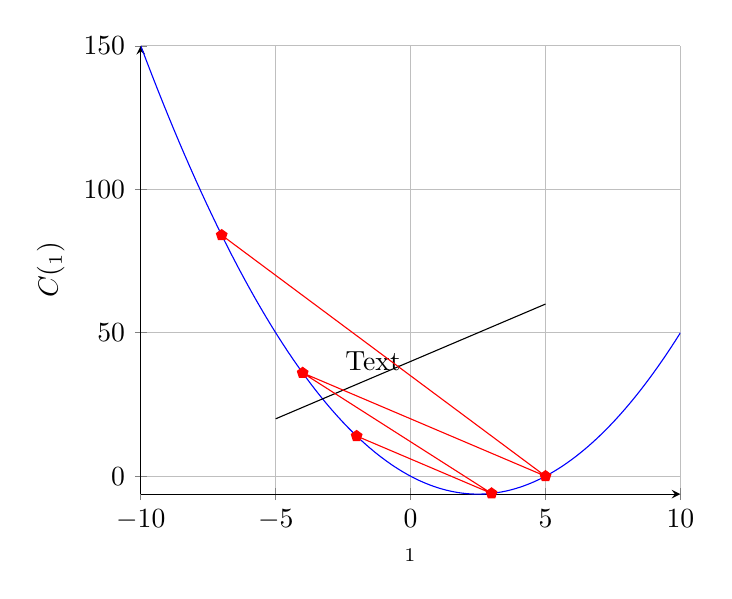
\begin{tikzpicture}
    \begin{axis}[
      axis lines = left,
      xlabel = $\param_1$,
      ylabel= {$C(\param_1)$},
      grid=major,
      ]
      \addplot [
      domain=-10:10,
      samples=100,
      color=blue
      ]
      {x^2 - 5*x};

      \draw (axis cs:-5,20) -- node[left]{Text} (axis cs:5,60);
      \addplot[color=red,mark=pentagon*,samples at={-7,5,-4,3,-2}] {x^2 - 5*x};

      \pgfmathparse{sin(60)}\pgfmathresult

    \end{axis}
  \end{tikzpicture}
  \caption{Visualisierung verschiedener Lernraten}
\end{figure}


\subsection{Stochastisches Gradientenverfahren fuer Machine Learning}
Wie vorhin erklaert, wird fuer das Trainieren eines Modells das Gradientenverfahren benutzt.
Konkret wird die Kostenfunktion $C(\vec{y},\vec{\hat{y}}\ |\ \param_0,\ldots,\param_n)$
($\param$ sind die Modellparameter, $\vec{y}$ die Vorhersagen und $\vec{\hat{y}}$
die Labels) minimieren, indem die Parameter angepasst werden. Dadurch macht das Modell immer bessere Vorhersagen.
Fuer nur eine Iteration des Gradientenverfahren, muesste man den Gradienten fuer den
\textit{gesamten} Trainingsdatensatz berechnen.
Dies waere zwar ein exakter Prozess, aber ein extrem langsamer zugleich.
Bei grossen Datensaetzen wuerde es eine Ewigkeit dauern, bis das Modell nur annahernd guete Vorhersagen machen wuerde.
\para{}
Aus diesem Grund verwendet man eine leicht abgeänderte Variante dieses
Verfahren, naemlich das \keyword{Stochastische Gradientenverfahren} (engl.:
Stochastic Gradient Descent) (SGD).
Hierfuer wird der ``echte'' Gradient des gesamten Datensatzes mit dem Gradienten einiger Trainingssamples approximiert.
Dazu wird der Trainingsdatensatz in sogennante \keyword{Mini-Batches} eingeteilt und der Gradient jeweils pro Mini-Batch berechnet.
Als Konsequenz finden deutlich mehr Iterationen statt in \textit{einer}
Durchkaemmung der Trainingsdaten. Eine solche Durchkaemmung bezeichnet man als
\keyword{Epoche}. Oft wird mehrere Epochen lang trainiert.
Der Gradient eines genug grossen Mini-Batches ist zwar nicht ganz exakt, aber approximiert den Gradieten des gesamten Datensatzen genuegend gut.
Sowohl die Mini-Batch Groesse, wie auch die Anzahl Epochen sind weitere Hyperparameter.
\para{}
Die partiellen Ableitungen der gesamten Trainingsdaten wird mit dem
arithmetischen Mittel der partiellen Ableitungen eines Mini-Batches der Groesse $q$ approximiert.
\\
\begin{equation}\label{eq:minibatch_deriv}
  \partderiv{\bar{C}}{\param_k} \approx \frac{1}{q}\sum_{i=1}^{q} \partderiv{C_i}{\param_k}
\end{equation}
\\
Eine Iteration des Stochastischen Graidentenverfahren wird analog zu Gleichung (\ref{eq:gradientdescent}) folgendermassen durchgefuehrt.
\\
\begin{equation}\label{eq:sgd}
  \param_{k,t+1} = \param_{k,t} - \frac{\eta}{q} \sum_{i=1}^{q} \partderiv{C_i}{\param_{k,t}}
\end{equation}


\subsection{Adam Optimizer?}

\section{Trainingsphaenomene}

\subsection{Overfitting}

% ------------------------------------------------------------

\chapter{Deep Learning und Künstliche Neuronale Netze}
Nun betrachten wir ein spezifisches Modell, welches die wohl besten Resultate
fuer die meisten Problemstellungen des Maschinelles Lernen (Bilderkennung,
Spracherkennung, etc.) liefert. Es handelt sich um das \keyword{Kuenstliche Neuronale Netz} (eng.: Neural Network) kurz KNN.
Der Bereich des Maschinelles Lernens, welcher sich mit Neuronalen Netzen
beschaeftigt, bezeichnet man als \keyword{Deep Learning}.
\para{}
Kuenstliche Neuronale Netze sind zum Teil biologisch von Nervensystemen vieler
Lebewesen inspiriert.
Sie sind aber lediglich eine Abstraktion ihrer Informationverarbeitung und versuchen nicht eine moeglichst genaue biologische Abbildung darzustellen.
Es gibt nicht nur eine Art von Neuralem Netz, sondern es exisitieren die
verschiedensten Architekturen, welche je nach Problemstellung ausgewaehlt werden
muessen. Diese Arbeit wird vorallem von zwei solchen Architekturen gebrauch machen:
Convolutional Neural Networks und sogennante Autoencodern.

\section{Perzeptron}
Um den Aufbau und die Funktion eines Kuenstlichen Neuronalen Netz besser zu
verstehen, wird im folgenden ein Vorgaenger des KNN erklaert: das \keyword{Perzeptron}.
\para{}
Das einlagige Perzeptron wurde erstmals 1958 von Frank Rosenblatt vorgestellt. Dieses
besteht aus einem einzigen Kuenstlichen Neuron. Dieses Kuenstliche Neuron
hat mehrere binaere Inputs und einen einzigen binaeren Output. Binaer
bedeutet, dass der Wert nur entweder 0 (\textit{aus}) oder 1 (\textit{ein}) sein
kann. Des weiteren besitzt es mehrere sogenannte \keyword{Gewichte} $w_1, \ldots,
w_m \in \set{R}$, fuer jeden Input $x_i$ ein Gewicht $w_i$.
Diese sind reelle Zahlen, welche das Verhalten des Perzeptron bestimmen.
Die \keyword{gewichtete Summe}, also die Summe aller Produkte der Inputs mit
ihrem Gewicht, wird mit $\tilde{z}$ bezeichnet.
Sie ist das gleiche wie das Skalarprodukt des Gewichtevektor
$\vec{w} = \trans{\begin{pmatrix} w_1 & \cdots & w_n \end{pmatrix}}$ mit dem
Inputvektor $\vec{x}$.
\\
\begin{equation*}
  \tilde{z} = \sum_{i=1}^{m} w_i x_i = \vec{w} \cdot \vec{x}
\end{equation*}
\\
Zusaetzlich besitzt das Perzeptron einen \keyword{Schwellenwert} $\tilde{b}$.
Zusammen mit den Gewichten, bilden sie die Modellparameter.
Das Perzeptron verhaelt sich so, dass falls die gewichtete Summe $\tilde{z}$ groesser als der
Schwellenwert $\tilde{b}$ ist, das Neuron feuert, d.h.\ der Output betraegt 1.
Andernfalls ist er 0 (siehe erster Teil der Hypothesenfunktion $h$ in Gleichung (\ref{eq:perzeptron_1})).
Es ist gaengig die Ungleichung der Bedingung in die Nullstellenform zu bringen
und $\tilde{b}$ durch die \keyword{Neigung} (engl.: Bias)
$b = -\tilde{b}$ zu ersetzten. Somit lautet die Ungleichung: $\tilde{z} + b
> 0$. Der neue Term $\tilde{z} + b$ wird mit $z$ bezeichnet (siehe Rest der Gl. (\ref{eq:perzeptron_1})).
Die Neigung gibt an wie stark das Neuron dazu neigt zu feuern. Eine grosse
Neigung laesst ein Neuron auch dann noch feuern, wenn nur wenige Inputs
eingeschaltet sind.
\\
\begin{equation}\label{eq:perzeptron_1}
  h(\vec{x}) =
  \begin{cases}
    1 & \quad \text{falls } \tilde{z} > \tilde{b}\\
    0 & \quad \text{ansonsten}
  \end{cases}
  \quad =
  \begin{cases}
    1 & \quad \text{falls } \tilde{z} + b > 0\\
    0 & \quad \text{ansonsten}
  \end{cases}
  \quad =
  \begin{cases}
    1 & \quad\text{falls } \vec{w} \cdot \vec{x} + b > 0\\
    0 & \quad\text{ansonsten}
  \end{cases}
\end{equation}
\\
\begin{figure}[h!]
  \centering
  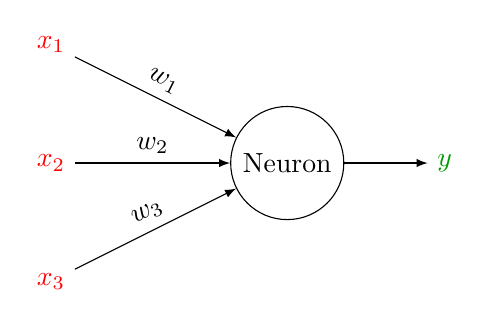
\begin{tikzpicture}[>=latex]
    \path (3,0) node [circle,draw](neuron){Neuron};
    \path[red] (0,1.5) node(x1){$x_1$} (0,0) node(x2){$x_2$} (0,-1.5) node(x3){$x_3$};
    \path[black!40!green] (5,0) node(y1){$y$};
    \draw[->] (x1) -- node[above,sloped]{$w_1$} (neuron);
    \draw[->] (x2) -- node[above,sloped]{$w_2$} (neuron);
    \draw[->] (x3) -- node[above,sloped]{$w_3$} (neuron);
    \draw[->] (neuron) -- (y1);
  \end{tikzpicture}
  \caption{Perzeptron mit drei Inputs}
  \label{fi:perzeptron}
\end{figure}
\\
Fuer das Trainieren des Perzeptron existieren spezielle Verfahren, welche hier
aber nicht relevant sind. Das Gradientenverfahren kann naemlich nicht verwendet
werden. Der Grund dafuer sollte spaeter in Sektion (\ref{sec:kuenstlicheNeuronen}) einleuchtend werden.

\subsection{Was kann ein Perzeptron erlernen?}
Nun stellt sich die Frage, was ein Perzeptron erlernen kann und wofuer es genutzt werden kann.
Das Perzeptron ist lediglich ein \keyword{Linearer Klassifikator} der Form
$y = w_1x_1 + \cdots + w_m x_m$. Es ist also ein Klassifizierungsmodell, kein Regressionsmodell.
Es kann die Features in zwei Klassen 0 oder 1 einordnen, wobei der Outputs der
Hypothesenfunktion, diese Klassifiezierung angibt.
Ueberschreitet $y$ den Schwellenwert, werden die Features der Klasse 1 zugeordnet, sonst
der Klasse 0.
Jedoch muessen diese Klassen linear separierbar sein.
\para{}
Lineare Separierbarkeit bedeutet, dass man alle Featurevektoren $\vec{x}_1,\ldots,\vec{x}_p \in \set{R}^m$
innerhalb ihres Vektorraums $\set{R}^m$ durch eine Hyperebene in ihre Klassen aufteilbar sein muessen.
Falls das Perzeptron zwei Inputs hat, bedeutet dies, dass die Ortsvektoren
einfach durch eine Gerade voneinander trennenbar sein muessen (siehe Abb.
(\ref{fig:linearer_Klassifikator})). \\
Falls die Features nicht linear separierbar sind, bedeutet dies, dass das
Perzeptron die Klassifizierung nicht erlernen kann.
BEISPIEL
\\
\begin{figure}[h!]
  \caption{erfolgreiche lineare Separierung (links) und das Versagen bei XOR (rechts)}
  \label{fig:linearer_Klassifikator}
\end{figure}
\para{}
\cite{wiki:perzeptron}
\cite{wiki:linear_separability}

\section{Erweiterung der Kuenstlichen Neuronen}\label{sec:kuenstlicheNeuronen}
Ein Perzeptron ist, wie vorhin erklaert, nur in der Lage, lineare Klassifikationen
durchzufuehren. Um nun auch kompliziertere Probleme zu loesen, muss das Prinzip
ausgebaut werden. Ausserdem brauchen wir ein Kuenstliches Neuron, welches sich
besonders gut als Baustein fuer KNNs eignet.

\subsection{Kuenstliche Neuronen im Allgemeinen}
Kuenstliche Neuronen sind immer so aufgebaut, dass sie einen oder mehrere Inputs
haben und einen einzigen Output. Zu jedem Input $x_i$ ist ein Gewicht
$w_{i}$ assoziert. Zuerst wird die gewichtete Summe der Inputs $\tilde{z}$ gebildet.
Die Neigung $b$ wird ebenfalls draufaddiert, um $z$ zu erhalten. Nun muss
die sogennante \keyword{Aktivierung} $a$ gebildet werden. Sie ist der Output des Neurons.
Die Aktivierung $a = \varphi(z)$ ist das Resultat der \keyword{Aktivierungsfunktion} $\varphi$ angewendet
auf $z$. Die verschiedenen Kuenstlichen Neuronen unterscheiden
sich fast nur in ihrer Aktivierungsfunktion.
\\
\begin{figure}[h!]

  \caption{ein kuenstliches Neuron und seine Bestandteile}
\end{figure}
\\

\subsection{Perzeptronen als Kuenstliche Neuronen}
Zuerst noch einmal ein Blick auf das Perzeptron im Angesicht der Aktivierungsfunktion.
Ein wesentlicher Unterschied des Perzeptron gegenueber sonstigen Kuenstlichen
Neuronen, besteht darin, dass seine Inputs und Outputs nur binaere Werte
annehmen koennen. Um dieses Verhalten des Perzeptron zu erhalten,
muss eine Stufenfunktion als Aktivierungfunktion verwendet werden: die Heaviside-Funktion $\Theta$.
Sie hat einen einzigen Stufensprung bei $x=0$ vom Wert 0 auf 1 (siehe Abb. (\ref{fig:heaviside})).
\\
\begin{figure}[h!]
  \begin{minipage}[h!]{0.5\textwidth}
    \begin{equation*}
      \varphi^{\text{hlim}}(z) = \Theta(z) =
      \begin{cases}
        1 & \quad \text{falls } z \geq 0\\
        0 & \quad \text{falls } z < 0
      \end{cases}
    \end{equation*}
  \end{minipage}
  \begin{minipage}[h!]{0.5\textwidth}
    \centering
    \begin{tikzpicture}[scale=2.5]
      \draw[->] (-1.5,0) -- (1.5,0) node[right] {$x$}; % x-axes
      \draw[->] (0,-0.2) -- (0,1.2) node [above] {$y$}; % y-axes
      \draw[style=help lines,step=0.5] (-1.4,0) grid (1.4, 1.1);

      \foreach \x in {-1,-0.5,0.5,1}
      \draw[shift={(\x,0)}] (0pt,2pt) -- (0pt,-2pt) node[below,fill=bgcolor] {$\x$};

      \foreach \y in {0.5,1}
      \draw[shift={(0,\y)}] (2pt,0pt) -- (-2pt,0pt) node[left,fill=bgcolor] {$\y$};

      \draw[shift={(0,0)}] (0pt,0pt) node[below left,fill=bgcolor] {$O$};

      \draw[red,ultra thick] (-1.5,0) -- (0,0); % 0-red
      \draw[red,ultra thick] (0,1) -- (1.5,1); % 1-red
      \draw[red,ultra thick,dashed] (0,0) -- (0,1); % y-red
      \draw[draw=red,fill=white] (0,0) circle (0.05);
      \draw[draw=red,fill=red] (0,1) circle (0.05);
    \end{tikzpicture}
  \end{minipage}
  \caption{Definition und Graph der Heaviside-Funktion $\Theta$}
  \label{fig:heaviside}
\end{figure}


\subsection{Stueckweise lineare Neuronen}
Der naechste Schritt nach dem binaeren Perzeptron sind sogenannte stueckweise
lineare Neuronen.
Sie verwenden eine stueckweise lineare Aktivierungsfunktion. Diese bildet ein
beschraenktes Intervall linear ab. Die Werte ausserhalb werden auf die
konstanten Werte 0 oder 1 abbgebildet (siehe Abb. (\ref{fig:stueckweiselinear})).
\para{}
Die Inputs koennen jetzt beliebige reelle Zahlen sein (vorzugsweise in der Naehe
von 0 und 1).
Ein KNN aus ausschliesslich linearen Neuronen ist ziemlich nutzlos, da jedliche Verkettung von
linearen Funktion auch durch eine einzige lineare Funktion dargestellt werden
koennte. Somit hat ein KNN gegenueber einem einzelnen Neuron keinen Mehrwert.
Ausserdem koennen mit diesen Neuron auch nur lineare Probleme geloest werden.
\\
\begin{figure}[h!]
  \begin{minipage}[h!]{0.5\textwidth}
    \begin{equation*}
      \varphi^{\text{pwl}}(z) =
      \begin{cases}
        1 & \quad \text{falls } z > \frac{1}{2}\\
        z + \frac{1}{2} & \quad \text{falls } -\frac{1}{2} < z < \frac{1}{2}\\
        0 & \quad \text{falls } z < \frac{1}{2}
      \end{cases}
    \end{equation*}
  \end{minipage}
  \begin{minipage}[h!]{0.5\textwidth}
    \centering
    \begin{tikzpicture}[scale=2.5]
      \draw[->] (-1.5,0) -- (1.5,0) node[right] {$x$}; % x-axes
      \draw[->] (0,-0.2) -- (0,1.2) node [above] {$y$}; % y-axes
      \draw[style=help lines,step=0.5] (-1.4,0) grid (1.4, 1.1);

      \foreach \x in {-1,-0.5,0.5,1}
      \draw[shift={(\x,0)}] (0pt,2pt) -- (0pt,-2pt) node[below,fill=bgcolor] {$\x$};

      \foreach \y in {0.5,1}
      \draw[shift={(0,\y)}] (2pt,0pt) -- (-2pt,0pt) node[left,fill=bgcolor] {$\y$};

      \draw[shift={(0,0)}] (0pt,0pt) node[below left,fill=bgcolor] {$O$};

      \draw[red,ultra thick] (-1.5,0) -- (-0.5,0); % 0-red
      \draw[red,ultra thick] (0.5,1) -- (1.5,1); % 1-red
      \draw[red,ultra thick] (-0.5,0) -- (0.5,1); % d-red

      \draw[draw=red,fill=red] (-0.5,0) circle (0.03);
      \draw[draw=red,fill=red] (0.5,1) circle (0.03);
    \end{tikzpicture}
  \end{minipage}
  \caption{Formel und Graph einer stueckweisen linearen Funktion}
  \label{fig:stueckweiselinear}
\end{figure}


\subsection{Sigmoide Neuronen}
Die logische naechste Erweiterung sind nicht-lineare Neuronen.
Ein sehr beliebter Kandidat dafuer sind Sigmoide Neuronen.
Den Namen haben sie von ihrer Aktivierungsfunktion: der Sigmoidfunktion $\sigma$.
Eine sehr wichtige Eigenschaft von ihr ist, dass sie - im Gegensatz zu den vorhin
genannten Aktivierungsfunktion - ueberall differenzierbar und strikt monoton
steigend ist. Erst fuer diese Aktivierungsfunktion, kann das Gradientenverfahren
angewendet werden und somit das KNN trainiert werden. Die anderen
Funktionen haben Stellen bei welchen die Ableitungsfunktion null
betraegt, somit kann das lokale Minimum nicht gefunden werden.
\para{}
Nicht nur die Sigmoidfunktion erfuellt diese Bedingungen, sondern auch andere. Die Sigmoidfunktion wird
bevorzugt, da ihre Ableitung sehr simpel ist (siehe Abb. (\ref{fig:sigmoid})).
Die Nicht-linearitaet dieser Neuronen ermoeglicht ein Erlernen von deutlich komplexeren Sachverhalten.
Und wie spaeter in Sektion (\ref{sec:UAT}) erlautert, ist es moeglich mit der Kompostion von nicht-linearen
Funktionen jede belibige Funktion zu approximieren!
\para{}
Die Sigmoid-Funktion besitzt eine einzige Wendestelle $\sigma''(x=0)=0$ und hat
zwei Asymptoten, eine $\ds\lim_{x \to -\infty} \sigma(x)=0$
und eine zweite $\ds\lim_{x \to \infty} \sigma(x)=1$ (siehe Abb. (\ref{fig:sigmoid})).
\\
\begin{figure}[h!]
  \begin{minipage}[h!]{0.5\textwidth}
    \begin{align*}
      \varphi^{\text{sig}}(z) &= \sigma(z) = \frac{1}{1 + e^{-z}}\\
      \sigma'(z)&=\sigma(z)(1-\sigma(z))
    \end{align*}
  \end{minipage}
  \begin{minipage}[h!]{0.5\textwidth}
    \centering
    \begin{tikzpicture}[scale=2.5]
      \draw[->] (-1.5,0) -- (1.5,0) node[right] {$x$}; % x-axes
      \draw[->] (0,-0.2) -- (0,1.2) node [above] {$y$}; % y-axes
      \draw[style=help lines,ystep=0.5,xstep=0.25] (-1.4,0) grid (1.4, 1.1);

      \foreach \x/\xtext in {-1/-4,-0.5/-2,0.5/2,1/4}
      \draw[shift={(\x,0)}] (0pt,2pt) -- (0pt,-2pt) node[below,fill=bgcolor] {$\xtext$};

      \foreach \y in {0.5,1}
      \draw[shift={(0,\y)}] (2pt,0pt) -- (-2pt,0pt) node[left,fill=bgcolor] {$\y$};

      \draw[shift={(0,0)}] (0pt,0pt) node[below left,fill=bgcolor] {$O$};

      \draw[red,ultra thick,x=0.25cm] plot[domain=-6.0:6.0] (\x,{1/(1+exp(-\x)) });
    \end{tikzpicture}
  \end{minipage}
  \caption{Definition, Ableitung und Graph der Sigmoid-Funktion $\sigma$}
  \label{fig:sigmoid}
\end{figure}


\section{Topologie der Kuenstlichen Neuronalen Netzen}
Nun sollten diese Sigmoiden Neuronen als Bausteine verwendet werden, um ein Kuenstliches
Neuronales Netz zu bilden. Dazu werden sie miteinander verbunden und bilden so ein Netz,
aehnlich wie ein Nervensystem.
\para{}
Diese Neuronen sind in verschieden Schichten (engl.: Layers)
arangiert. Die erste ist die \keyword{Inputschicht}. Sie behinhalten die
Inputneuronen. Diese sind eigentlich keine richtigen
Neuronen sondern eher Platzhalter fuer ihr jeweiliges Feature $x_i$. Als letztes kommt die
\keyword{Outputschicht} mit den Outputneuronen, welche jeweils einen Outputwert $y_i$
besitzen. Dazwischen liegen die \keyword{Zwischenschichten} (engl.: Hiddenlayer). Von ihnen kann es
beliebig viele geben und in ihnen beliebig viele Neuronen.
Falls viele Zwischenschichten verwendet werden, bezeichnet man das Netzwerk als
``deep''. Daher ruert auch der Name des Deep Learnings.
Der Aufbau eines KNN bezeichnet man als \keyword{Topologie} des Netzes. Die
Topologie umfasst viele Hyperparameter. Darunter sind zum Beispiel die Anzahl Zwischenschichten, wie auch
die Anzahl Neuronen pro Schicht.
\para{}
Jedes Neuron aus einer Schicht ist mit jedem Neuron aus der naechsten Schicht ueber
Verbindungen gekoppelt. Alle Verbindungen besitzten ein Gewicht analog zu den Inputs des
Perzeptron. Die Aktivierung, also der Output, eines Neurons wandert entlang den jeweiligen
Verbindung zu allen Neuronen der naechsten Schicht und dient als deren Input.
Die soeben beschriebe Art von KNN nennt man \keyword{Feedforward-Netz}, da alle Werte
ausschliesslich nach vorne propagiert werden.
\para{}
In Abbildung (\ref{fig:nn_layers}) ist ein Beispiel eines Neuronalen Netzes
abgebildet. In diesem Fall besitz es sowohl 4 Inputs, wie auch 4 Outputs. Es hat
ausserdem 3 Zwischenschichten. Die erste und die dritte haben jeweils 3 Neuronen
und die zweite besitzt 4 Neuronen. \\

\begin{figure}[h!]
  \centering
  \begin{tikzpicture}[>=latex]

    \tikzstyle{netstyle} = [matrix of nodes,nodes={draw,circle,inner sep=0, minimum size=1cm},column sep=0.5cm,row sep=-9pt]
    \tikzstyle{cl} = [draw=none,fill=none]
    \tikzstyle{heading} = [clear,text width=15mm,text centered]
    \tikzstyle{inp} = [fill=red!70!bgcolor]
    \tikzstyle{hid} = [fill=blue!70!bgcolor]
    \tikzstyle{ou} = [fill=green!70!bgcolor]

    \matrix[netstyle] (mat)
    {
      |[inp]| $x_1$     & |[cl]| & |[cl]| & |[hid]|$h_1^2$ & |[cl]| & |[cl]| & |[ou]|$y_1$ \\
      |[cl]| & |[cl]| & |[hid]|$h_1^1$   & |[cl]| & |[hid]|$h_1^3$ & |[cl]| & |[cl]| \\
      |[inp]| $x_2$     & |[cl]| & |[cl]| & |[hid]|$h_2^2$ & |[cl]| & |[cl]| & |[ou]|$y_2$ \\
      |[cl]| & |[cl]| & |[hid]|$h_2^1$   & |[cl]| & |[hid]|$h_2^3$ & |[cl]| & |[cl]| \\
      |[inp]| $x_3$     & |[cl]| & |[cl]| & |[hid]|$h_3^2$ & |[cl]| & |[cl]| & |[ou]|$y_3$ \\
      |[cl]| & |[cl]| & |[hid]|$h_3^1$   & |[cl]| & |[hid]|$h_3^3$ & |[cl]| & |[cl]| \\
      |[inp]| $x_4$     & |[cl]| & |[cl]| & |[hid]|$h_4^2$ & |[cl]| & |[cl]| & |[ou]|$y_4$ \\
    };

    % titels
    \node [yshift=1cm] at (mat-1-1) {Inputschicht};
    \node [yshift=1cm] at (mat-1-4) {Zwischenschichten};
    \node [yshift=1cm] at (mat-1-7) {Outputschicht};

    % dots
    % \node [yshift=-1cm,scale=2] at (mat-7-1) {$\vdots$}; % for inputs
    % \node [yshift=-1cm,scale=2] at (mat-6-3) {$\vdots$};
    % \node [yshift=-1cm,scale=2] at (mat-7-4) {$\vdots$};
    % \node [yshift=-1cm,scale=2] at (mat-6-5) {$\vdots$};
    % \node [yshift=-1cm,scale=2] at (mat-7-7) {$\vdots$}; % for outputs

    % input -> hidden1
    \foreach \ai in {1,3,...,7} {
      \foreach \aii in {2,4,6}
      \draw[->] (mat-\ai-1) -- (mat-\aii-3);
    }

    % hidden1 -> hidden2
    \foreach \ai in {2,4,...,6} {
      \foreach \aii in {1,3,...,7}
      \draw[->] (mat-\ai-3) -- (mat-\aii-4);
    }

    % hidden2 -> hidden3
    \foreach \ai in {1,3,...,7} {
      \foreach \aii in {2,4,6}
      \draw[->] (mat-\ai-4) -- (mat-\aii-5);
    }

    % hidden3 -> output
    \foreach \ai in {2,4,...,6} {
      \foreach \aii in {1,3,...,7}
      \draw[->] (mat-\ai-5) -- (mat-\aii-7);
    }


  \end{tikzpicture}
  \caption{Schichten eines KNNs}
  \label{fig:nn_layers}
\end{figure}

\section{Lernverhalten}
Die Hoffnung beim Trainieren von KNNs besteht darin, dass das Modell fuer jede
weiter Schicht eine hoeheres Abstraktionsniveau erreicht. Wuerde man zum
Beispiel ein Netzwerk zur Gesichtserkennung trainieren, koennte man sich den
Erkennungsprozess folgendermassen vorstellen. Die erste Zwischenschicht erkennt
Kanten und Konturen. Die zweite vereint diese Merkmale zu Ecken und primitive
geometrische Formen. Die dritte Schicht sollte dann schon komplexere
geometrische Formen erkennen, welche gewissen Gesichtmerkmalen, wie der Nase, aehneln. Die letzten Schichten sollte dann all diese
Merkmale zusammensetzen und so ein Gesicht erkennen.
WEITERFUEHREN

\section{Vorwaertspropagierung}
Jetzt, da der Aufbau eines KNNs erklaert wurde, sollte nun die mathematische Funktionsweise
des Modells erklaert werden. Hierfuer muessen einige Konventionen zur
Bezeichnung der Teile eines KNNs getroffen werden. Es sollten vorallem noch
Abbildungen (\ref{fig:nomenklatur1}) und (\ref{fig:nomenklatur2}) zum Verstaentniss der Nomenklatur studiert werden.
\begin{itemize}
\item{$l$ ist der Index einer Schicht. Die Indexierung beginnt bei 0.}
\item{$L$ ist der letzte Schichtindex und somit auch die gesamte Anzahl an Schichten.}
\item{$|l|$ ist die Anzahl Neuronen in der $l$-ten Schicht.
    \footnote{
      Diese Schreibweise hat nichts mit dem Betrag zu tun, sondern wird einfach
      gewaehlt, da sie sehr platzsparend ist.
    }
  }
\item{$n_j^l$ ist das $j$-te Neuron in der $l$-ten Schicht.}
\item{$z_j^l$ ist die gewichtete Summe der Inputs des $j$-ten Neuron in der $l$-ten Schicht.}
\item{$a_j^l$ ist die Aktivierung/Output des $j$-ten Neurons in der $l$-ten Schicht.}
\item{$b_j^l$ ist die Neigung fuer das $j$-te Neuron in der ($l+1$)-ten Schicht.
    \footnote{
      Diese Konvention wurde gewaehlt, damit die folgenden Gleichungen simpler sind.
    }
  }
\item{$w_{j,k}^l$ ist das Gewicht der Verbindung vom $k$-ten Neuron
    in der $l$-ten Schicht zum $j$-ten Neuron in der ($l+1$)-ten Schicht.
    \footnote{
      Man beachte die Reihenfolge!\\
      Diese Konvention scheint zwar auf den ersten Blick unintuitiv, macht jedoch
      Sinn fuer die Matrixindezierung.
      (\ref{sec:backpropagation}).
    }
  }
\item{$\varphi$ ist die gewaehlte Aktivierungsfunktion (grundsaetzlich ist diese
    immer die Sigmoidfunktion $\sigma$).}
\end{itemize}

\begin{figure}[h!]
  \centering
  \begin{tikzpicture}[>=latex]
    \tikzstyle{netstyle} = [matrix of nodes,nodes={draw,circle,inner sep=0, minimum size=1.25cm},column sep=0.5cm,row sep=-9pt]
    \tikzstyle{cl} = [draw=none,fill=none]
    \tikzstyle{sy} = [cl,font=\LARGE]
    \tikzstyle{heading} = [clear,text width=15mm,text centered]
    \tikzstyle{inp} = [fill=red!70!bgcolor]
    \tikzstyle{hid} = [fill=blue!70!bgcolor]
    \tikzstyle{ou} = [fill=green!70!bgcolor]

    \matrix[netstyle] (mat)
    {
      |[inp]|$n_1^0$     & |[cl]| & |[cl]| & |[cl]| & |[cl]| & |[cl]| & |[ou]|$n_1^L$ \\
      |[cl]| & |[cl]| & |[hid]|$n_1^1$   & |[sy]| $\cdots$ & |[hid]|$n_1^{L-1}$ & |[cl]| & |[cl]| \\
      |[inp]|$n_2^0$     & |[cl]| & |[cl]| & |[cl]| & |[cl]| & |[cl]| & |[ou]|$n_2^L$ \\
      |[cl]| & |[cl]| & |[hid]|$n_2^1$   & |[sy]| $\cdots$ & |[hid]|$n_2^{L-1}$ & |[cl]| & |[cl]| \\
      |[inp]|$n_3^0$     & |[cl]| & |[sy]| $\vdots$ & |[cl]| & |[sy]| $\vdots$ & |[cl]| & |[ou]|$n_3^L$ \\
      |[sy]| $\vdots$ & |[cl]| & |[hid]|$n_{|1|}^1$ & |[sy]|$\cdots$ & |[hid]|$n_{|L-1|}^{L-1}$ & |[cl]| & |[sy]| $\vdots$ \\
      |[inp]|$n_{|0|}^0$ & |[cl]| & |[cl]| & |[cl]| & |[cl]| & |[cl]| & |[ou]|$n_{|L|}^L$ \\
    };

    % titels
    \node [yshift=1.5cm] at (mat-1-1) {Inputschicht};
    \node [yshift=1.5cm] at (mat-2-4) {Zwischenschichten};
    \node [yshift=1.5cm] at (mat-1-7) {Outputschicht};

    % input -> hidden1
    \foreach \ai in {1,3,...,7} {
      \foreach \aii in {2,4,...,6}
      \draw[->] (mat-\ai-1) -- node[above,sloped]{} (mat-\aii-3);
    }

    % hidden1 ->...
    \foreach \ai in {2,4,...,6} {
      \foreach \aii in {2,4,...,6} {
        \node (A) at (mat-\ai-3) {};
        \node (B) at (mat-\aii-5) {};
        \draw[left color=black,right color=white] (mat-\ai-3) -- ($(A)!0.3!(B)$);
      }
    }

    % ...-> hidden2
    \foreach \ai in {2,4,...,6} {
      \foreach \aii in {2,4,...,6} {
        \node (A) at (mat-\ai-3) {};
        \node (B) at (mat-\aii-5) {};
        \draw[left color=black,right color=white] ($(A)!0.7!(B)$) -- (mat-\aii-5);
      }
    }

    % hidden3 -> output
    \foreach \ai in {2,4,...,6} {
      \foreach \aii in {1,3,...,7}
      \draw[->] (mat-\ai-5) -- node[above,sloped]{} (mat-\aii-7);
    }

    \node[below=2mm of mat-7-1.south] {$l=0$};
    \node[below=2mm of mat-6-3.south] {$l=1$};
    \node[below=2mm of mat-6-5.south] {$l=L-1$};
    \node[below=2mm of mat-7-7.south] {$l=L$};
  \end{tikzpicture}
  \label{fig:nomenklatur1}
  \caption{zum Verstaentniss der Nomenklatur}
\end{figure}
\para{}
\begin{figure}[h!]
  \centering
  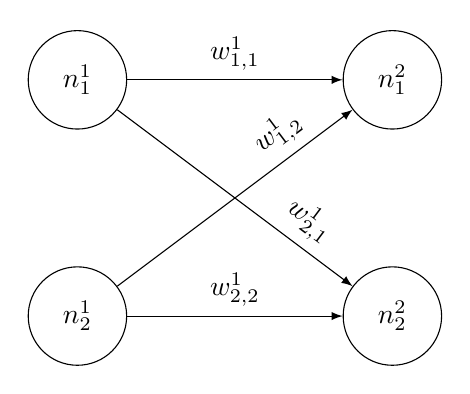
\begin{tikzpicture}[>=latex]
    \path (-2,1.5) node [draw,circle,inner sep=0,minimum size=1.25cm](n11){$n^1_1$};
    \path (-2,-1.5) node [draw,circle,inner sep=0,minimum size=1.25cm](n12){$n^1_2$};
    \path (2,1.5) node [draw,circle,inner sep=0,minimum size=1.25cm](n21){$n^2_1$};
    \path (2,-1.5) node [draw,circle,inner sep=0,minimum size=1.25cm](n22){$n^2_2$};
    \draw[->] (n11) -- node[above,sloped]{$w^1_{1,1}$} (n21);
    \draw[->] (n11) -- node[above,pos=0.75,sloped]{$w^1_{2,1}$} (n22);
    \draw[->] (n12) -- node[above,pos=0.75,sloped]{$w^1_{1,2}$} (n21);
    \draw[->] (n12) -- node[above,sloped]{$w^1_{2,2}$} (n22);
  \end{tikzpicture}
  \label{fig:nomenklatur2}
  \caption{zum Verstaentniss der Gewichtebeschriftungen}
\end{figure}
\para{}
Die Vorwaertspropagierung beginnt bei den Inputneuronen, welche jeweils
einen Inputwert in sich tragen. Diese werden, um fuer eine kohaerente Nomenklatur zu sorgen,
analog zu den Aktivierungen der anderen Neuronen mit $a_j^0$ bezeichnet, wobei
$j$ der Index des Neurons ist. \\
Nun muessen die restlichen Aktivierungen der Neuronen bis und mit den Ouputneuronen berechnet werden. Dies geschieht rekursiv, anhand der
Aktivierungen der voherigen Schicht. Und zwar folgendermassen (ersichtlich in
Gleichung (\ref{eq:gewichtete_summe_normal})).
\para{}
Zuerst laueft eine Summe ueber alle Neuronen $n_k^{l}$ der jetztigen Schicht
$l$. Dabei wird die gewichtete Summe der Aktivierungen $a_k^{l}$ mit den
assozierten Gewichten $w_{j,k}^l$ gebildet. Hierbei ist das Gewicht jenes, welches das
$k$-te Neuron der $l$-ten Schicht mit dem $j$-ten Neuron der ($l+1$)-ten Schicht verbindet.
Zusaetzlich gehoert zu der gewichteten Summe auch die jeweilige Neigung $b_j^l$, welche
dazuaddiert wird. Diese gewichtete Summe wird mit $z_j^{l+1}$ bezeichnet.
\\
\begin{equation}\tag{FP1}\label{eq:gewichtete_summe_normal}
  z_j^{l+1} = \sum_{k=1}^{|l|} w_{j,k}^l a_k^l + b_j^l
\end{equation}
\\
Auf diese Summe wird dann die Aktivierungsfunktion $\varphi$ angewandt.
Das ist dann die Aktivierung $a_j^{l+1}$ des $j$-ten Neurons in der ($l+1$)-ten Schicht.
\\
\begin{equation}\tag{FP2}\label{eq:aktivierung_normal}
  a_j^{l+1} = \varphi\left(\sum_{k=1}^{|l|} w_{j,k}^l a_k^{l} + b_j^l \right) = \varphi \left( z_j^{l+1} \right)
\end{equation}
\par\bigskip
Fuer Deep Learning braucht man vorallem sogennante Deep Neural Networks. Diese
zeichnen sich dadurch aus, dass sie sehr viele Zwischenschichten besitzen.
Deshalb bezeichnet man sie auch als ``deep''.
Bei solchen Netzwerken ist es nicht unueblich,
dass diese sehr viele Neuronen und Verbindungen (ueber 100'000) besitzen.
Um hierbei nicht den Ueberblick zu verlieren und um nicht in den Indizes zu
ertrinken, macht man Gebrauch von \keyword{Linearer Algebra}. Man verwendet
Matrizen und Vektoren um die vielen Variabeln zusammenzufassen.
Ausserdem besteht ein weiterer Vorteil darin, dass Computer mithilfe von Vektor-
und Matrixoperationen die Berechnungen parallisieren koennen und in kuerzerer
Zeit und mit weniger Ressourcen viele Berechnungen gleichzeitig ausfuehren koennen.
Dies beschleunigt das Training der Modelle um
ein Vielfaches. Dies wird spaeter in Sektion
(\ref{sec:tensorflow}) noch weiter thematisiert.
\para{}
Die Inputs $\vec{x}$, Vorhersagen $\vec{y}$ und Labels $\vec{\hat{y}}$ haben wir schon von Anfang an als Vektoren geschrieben.
Nun sollen noch die Modellparameter und die restlichen Komponenten eines KNNs als Vektoren und Matrizen zusammengefasst werden.
Sowohl alle gewichteten Summen $z_j^l$, wie auch alle Aktivierungen $a_j^l$
einer Schicht $l$, werden in Vektoren $\vec{z}^l \in \set{R}^{|l|}$ und
$\vec{a}^l \in \set{R}^{|l|}$ zusammengefasst.
Auch alle Neigung $b_j^l$ fuer eine Schicht ($l+1$) bilden einen Vektor
$\vec{b}^l \in \set{R}^{|l+1|}$.
\para{}
Zu guter letzt, wird noch eine \keyword{Gewichtsmatrix} $\mat{W}^l \in
\set{R}^{|l+1| \times |l|}$
definiert. Sie enthaltet alle Gewichte welche die $l$-te
Schicht \textit{zu} der ($l+1$)-ten Schicht verbindet.
Das heisst der Eintrag in der $j$-ten Zeile und in
der $k$-ten Spalte ist $w_{j,k}^l$ und verbindet so das Neuron $n_k^{l}$ zu
dem Neuron $n_j^{l+1}$.
\\
\begin{align*}
  \vec{z}^l &=  \trans{\begin{pmatrix} z_1^l & z_2^l & \cdots & z_{|l|}^l \end{pmatrix}} \\
  \vec{a}^l &=  \trans{\begin{pmatrix} a_1^l & a_2^l & \cdots & a_{|l|}^l \end{pmatrix}} \\
  \vec{b}^l &=  \trans{\begin{pmatrix} b_1^l & b_2^l & \cdots & b_{|l+1|}^l \end{pmatrix}} \\
\end{align*}
\begin{equation*}
  \mat{W}^l =
  \begin{pmatrix}
    w_{1,1}^l & w_{1,2}^l & \cdots & w_{1,|l|}^l \\[0.3em]
    w_{2,1}^l & w_{2,2}^l & \cdots & w_{2,|l|}^l \\[0.3em]
    \vdots & \vdots & \ddots & \vdots \\[0.3em]
    w_{|l+1|,1}^l & w_{|l+1|,2}^l & \cdots & w_{|l+1|,|l|}^l
  \end{pmatrix}
\end{equation*}
\\
Mit diesen Definitionen kann nun Gleichung (\ref{eq:gewichtete_summe_normal}) in
Matrixform geschrieben werden, denn die Matrixmultiplikation von $\mat{W}^l$ mit
$\vec{a}^{l}$ ergibt einen Vektor $\vec{\tilde{z}}^{l+1}$, welcher alle gewichteten
Summen $\tilde{z}_j^{l+1}$ ohne die jeweilige Neigung enthaelt.
\\
\begin{equation*}
  \mat{W}^l \vec{a}^{l} = \trans{\begin{pmatrix}\ds \sum_{j=1}^{|l|} w_{1,j}^l a_j^l &\ds \sum_{j=1}^{|l|} w_{2,j}^l a_j^l & \cdots &\ds \sum_{j=1}^{|l|} w_{|l+1|,j} a_j^l \end{pmatrix}} = \vec{\tilde{z}}^{l+1}
\end{equation*}
\\
Nun muessen wir noch den Neigungsvektor $\vec{b}^l$ draufaddieren und wir
erhalten Gleichung (\ref{eq:gewichtete_summe_matrix}), mithilfe dessen wir den
Vektor der gewichteten Summen $\vec{z}^{l+1}$ bilden koennen.
\\
\begin{equation}\tag{FP1a}\label{eq:gewichtete_summe_matrix}
  \vec{z}^{l+1} = \mathbf{W}^{l} \vec{a}^{l} + \vec{b}^{l}
\end{equation}
\\
Der letzte Schritt besteht noch darin die Aktivierungsfunktion auf $\vec{z}^{l+1}$
anzuwenden um den Aktivierungsvektor $\vec{a}^{l+1}$ zu bilden.
Hierfuer muss aber noch ein neues mathematisches
Konzept eingefuehrt werden: die Vektorisierung einer Funktion.
\para{}

\begin{defbox}{Vektorisierung einer Funktion}
  Die Vektorisierung einer skalaren Funktion $f$, geschrieben als
  $\vecf{f}[\vec{v}]$ hat als Argument einen Vektor $\vec{v}$, auf dessen
  Komponenten jeweils \textit{einzeln} die Funktion $f$ angewandt wird. Dieser neue
  Vektor ist der Rueckgabewert der Funktion. Er besitzt die gleichen Dimensionen
  wie der Argumentvektor.
  \\
  \begin{equation*}
    \vecf{f}[\vec{v}]=
    \begin{pmatrix}
      f(v_1)\\
      \vdots \\
      f(v_n)\\
    \end{pmatrix}
  \end{equation*}
\end{defbox}

Nun kann ganz einfach die vektorisierte Aktivierungsfunktion $\vecf{\varphi}$ auf
$\vec{z}^{l+1}$ angewandt werden.

\begin{equation}\tag{FP2a}\label{eq:aktivierung_matrix}
  \vec{a}^{l+1} = \vecf{\varphi} \left[\mat{W}^{l} \vec{a}^{l} + \vec{b}^{l} \right] = \vecf{\varphi} \left[ \vec{z}^{l+1} \right]
\end{equation}

\para{}
\cite{Nielsen}

\subsection{Modellparameter initalisieren}\label{sec:parameter_initalisieren}
Ein Schritt der getan werden muss, bevor das Training beginnt, ist das
Initalisieren aller Modellparameter, in diesem Fall die Gewichte und Neigungen.
Dies ist ein sehr essentieller Schritt, denn diese Startwerte entscheiden
erheblich ueber die Leistungsfaehigkeit des Modells.
\para{}
Wie in Sektion (\ref{sec:gradientenverfahren}) gezeigt, muss am Anfang des
Gradientenverfahrens ein Startpunkt $\vec{p}_0$ innerhalb des Gradientenfeldes
$\vecf{\nabla}C$ gewaehlt werden, von welchem aus der Gradientenabstieg beginnt.
Da wir das Gradientenverfahren zur Optimierung der Modellparameter verwenden,
ist unser Startpunkt, der Vektor aller Hyperparameter
$\vec{\param} = \trans{\begin{pmatrix} \param_1 & \cdots & \param_k \end{pmatrix}}$.
Dieser Startpunkt entscheidet darueber, in welches lokale Minimum konvergiert
wird und bestimmt somit auch die bestmoegliche Exaktheit der Vorhersagen. Falls
schlecht Initalwerte gewaehlt werden, konvergiert der Punkt in ein hohes lokales
Minimum, was grosse Kostenfunktionswerte und schlecht Vorhersagen verursacht.
\para{}
Es ist nicht moeglich im Vorhinein zu wissen, welche Initalwerte gute Resultate
liefern. Man muss ausprobieren, deshalb initalisert man gaengierweise die
Hyperparameter mit Zufallswerten. Dafuer nimmt man aber nicht irgendwelche
Zufallsvariablen sondern man benutzt die Gauss'sche Normalverteilung
$\mathcal{N}(\mu,\sigma^2)$ bzw. ihre Dichtefunktion
\[\ds \phi(x\ |\ \mu,\sigma^2) = \frac{1}{\sqrt{2\pi\sigma^2}} \text{exp} \left\{-\frac{{(x-\mu)}^2}{2\sigma^2}\right\} \]
\para{}

\ifcp
\pgfplotsset{compat=1.15}
\pgfmathdeclarefunction{gauss}{2}{%
  \pgfmathparse{1/(#2*sqrt(2*pi))*exp(-((x-#1)^2)/(2*#2^2))}%
}
\pgfmathdeclarefunction{gausseval}{3}{%
  \pgfmathparse{1/(#2*sqrt(2*pi))*exp(-((#3-#1)^2)/(2*#2^2))}%
}
\usetikzlibrary{arrows.meta}    % <--- added

\begin{figure}[h!]
  \centering
  \begin{tikzpicture}[
    every pin/.style = {pin edge={Latex-,thin,black}},>=latex
    ]
    \begin{axis}[
      width=15cm,height=6cm,
      scale only axis,
      axis lines=middle,
      ymin=0,ymax=0.45,
      axis line style = thick,
      xtick={-3,-2,-1,1,2,3},
      x label style={anchor=west},
      y label style={anchor=south},
      extra x ticks={0},
      extra x tick style={%
        grid=major,
        ticklabel pos=top,
      },
      extra x tick labels={$\mu$},
      xlabel={$x$},
      ylabel={$\phi(x)$},
      axis on top,
      samples=50]
      \addplot[pattern=north west lines,pattern color=blue!25,domain=-3.5:3.5] {gauss(0,1)} \closedcycle;
      \addplot[domain=-3.5:3.5,red,thick] {gauss(0,1)};
      \coordinate (wp1) at (-1,{gausseval(0,1,-1)});
      \coordinate (wp2) at (1,{gausseval(0,1,1)});
      \coordinate (zero) at (0,0);
      \newcommand{\equal}{=}
      % \path [fill=black] (wp1) circle (2pt);
      % \path [fill=black] (wp2) circle (2pt);
      \path [draw=black,<->,very thick] (wp1) -- node[above]{$\sigma^2$} (wp1 -| zero);
      \path [draw=black,<->,very thick] (wp2) -- node[above]{$\sigma^2$} (wp2 -| zero);
      \node [pin=120:$\phi(x_{WS1})'' \equal 0$] at (wp1) {};
      \node [pin=60:$\phi(x_{WS2})'' \equal 0$] at (wp2) {};

      \node [pin=60:$\ds A \equal \int_{-\infty}^{\infty} \phi(x) \text{d}x \equal 1$] at (1.4,0.05) {};
    \end{axis}
  \end{tikzpicture}
  \caption{Graph der Dichtefunktion $\phi(x\ |\ \mu=0,\sigma^2=1)$ mit ihren
    wichtigsten Eigenschaften}%
\end{figure}
\fi


Um die Neigungen $b_{t=0}$ zu initalisieren benutzt man eine Normalverteilung
$\mathcal{N}(0,1)$ mit Erwartungswert $\mu = 0$ und Varianz $\sigma^2 =
1$. Um die Gewichte $w_{t=0}$ zu initalisieren benutzt man ebenfalls eine
Normalverteilung mit Erwartungswert $\mu = 0$, jedoch wird die Varianz
$\sigma^2$ so skaliert, dass die Summe aller Zufallesvariabeln der Gewichte
einer Schicht eine Varianz von $\sigma^2_{tot} = 1$ hat.
\begin{align}
  w_{t=0}^l &\sim \mathcal{N}(\mu = 0, \sigma^2 = \frac{1}{|l|}) \\
  b_{t=0}^l &\sim \mathcal{N}(\mu = 0, \sigma^2 = 1)
\end{align}


\para{}
\cite{wiki:normal_distribution}
\cite{Nielsen}

\section{Rueckwaertspropagierung}\label{sec:backpropagation}
Die wahre Herausforderung besteht beim Gradientenverfahren darin,
die partiellen Ableitungen der Modellparameter,
also die Komponenten des Gradienten, zu bestimmen.
Anderst gesamt muessen alle Terme
$\ds\partderiv{C}{w_{j,k}^l}$, wie auch alle Terme $\ds\partderiv{C}{b_k^l}$
berechnet werden.
Das Verfahren zum bestimmen dieser Ausdruecke ist so spezfisch und aufwendig,
dass das Gradientenverfahren fuer KNNs einen eigenen Namen hat: die
\keyword{Rueckwaertspropagierung} (engl.: Backpropagation) (auch Fehlerrueckfuehrung).
\para{}
Da ein KNN, wie der Name es schon sagt, vernetzt ist, koennen die partiellen
Ableitungen einer Schicht bezueglich seiner Nachbarsschichten berechnet werden.
Dies ist auch der namensgebende Grundgedanke der Rueckwaertsprogagierung: Man
beginnt in der letzten Schicht die partiellen Ableitungen zu bestimmen und
berechnet dann im Rueckwaertsgang Schicht fuer Schicht die vorherigen
partiellen Ableitungen, bis nach vorne. \\
Dies macht man mithilfe der Kettenregel der Ableitungen.
Es ist sinnvoll fuer das Aufstellen dieser Gleichungen das Netzwerk als
\keyword{Computation Graph} zu betrachten.
\para{}
Ein Computation Graph ist eine Darstellung einer Verkettung von Funktionen als Netzwerk von Operationen.
Die Knoten im Graph stellen Variabeln dar und die Pfade, welche die Knoten
verbinden, sind die Funktionen, welche die Variabeln aufeinander abbilden. Die
Funktion wird auf die Variable angewandet, von der der Pfad ausgeht. Der Knoten
in welchem der Pfad endet, nimmt dann den Funktionswert an. Falls
mehrere Pfade in einem Knoten enden, werden die einzelnen Werte der Pfade
zusammenaddiert, um die Variable zu bilden. \\
In Abbildung (\ref{fig:computation_graph}) ist ein Beispiel eines Computation
Graphs zusammen mit der Herleitung der partiellen Ableitungen dargestellt.
\para{}
\begin{figure}[h!]
  \begin{minipage}[h!]{0.5\textwidth}
    \centering
    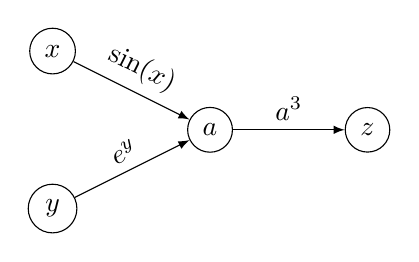
\begin{tikzpicture}[>=latex]

      \path (0,1) node [circle,draw](var_x){$x$};
      \path (0,-1) node [circle,draw](var_y){$y$};
      \path (2,0) node [circle,draw](var_a){$a$};
      \path (4,0) node [circle,draw](var_z){$z$};
      % \path[red] (0,1.5) node(x1){$x_1$} (0,0) node(x2){$x_2$} (0,-1.5) node(x3){$x_3$};
      \draw[->] (var_x) -- node[above,sloped]{$\sin(x)$} (var_a);
      \draw[->] (var_y) -- node[above,sloped]{$e^y$} (var_a);
      \draw[->] (var_a) -- node[above,sloped]{$a^3$} (var_z);

    \end{tikzpicture}

  \end{minipage}
  \begin{minipage}[h!]{0.5\textwidth}
    \begin{align*} % or align*
      a(x,y) &= \sin(x) + e^y \\
      z(a(x,y)) &= a^3(x,y) = \left(\sin(x) + e^y\right)^3 \\[3ex]
      \partderiv{z}{x} &= \partderiv{a}{x} \cdot  \partderiv{z}{a} = \cos(x) \cdot 3a^2 \\[0.5ex]
      \partderiv{z}{y} &= \partderiv{a}{y} \cdot \partderiv{z}{a} = e^y \cdot 3a^2
    \end{align*}
  \end{minipage}

  \caption{Computation Graph einer exemplarischen Verkettung von Funktionen}
  \label{fig:computation_graph}
\end{figure}
\para{}
Der erste Schritt der Rueckwaertsprogagierung besteht darin, dass man die partiellen Ableitungen $\ds\partderiv{C}{z_j^l}$
der Kostenfunktion $C$ bezueglich den gewichteten Summen $z_j^l$ aller Schichten
berechnet. Daraus laesst sich dann spaeter sehr einfach die partiellen Ableitungen
bezueglich den Gewichten $\ds\partderiv{C}{w_{j,k}^l}$ und bezueglich den Neigung
$\ds\partderiv{C}{b_j^l}$ berechnen.
\para{}
Zur Uebersichtlichkeit definiert man einen \keyword{Fehler} $\delta_j^L$ fuer
jedes $j$-te Neuron in jeder $l$-ten Schicht, welcher die partielle Ableitung bezueglich der
gewichteten Summe ist (siehe Gl. (\ref{eq:BP0)}). Ebenfalls definiert man analog einen Fehlervektor
$\vec{\delta}^l$, welcher alle Fehler $\delta_j^l$ einer Schicht $l$
zusammenfasst (siehe Gl. (\ref{eq:BP0a})). Nun heisst es diesen fuer jedes Neuron jeder Schicht zu
berechnen.
\\
\begin{gather}
  \tag{BP0}\label{eq:BP0} \delta_j^l \coloneqq \partderiv{C}{z_j^l} \\
  \tag{BP0a}\label{eq:BP0a} \vec{\delta}^l \coloneqq \trans{\begin{pmatrix} \ds\partderiv{C}{z_1^l} & \ds\partderiv{C}{z_2^l} & \cdots & \ds\partderiv{C}{z_{|l|}^l} \end{pmatrix}}
\end{gather}
\\
Da die Kostenfunktion unmittelbar auf die letzte Schicht $L$ angewandt wird, beginnt
man auch dort mit der Berechnung des Fehlers $\vec{\delta}^L$.
Wir stellen nun einen Computation Graph auf, um die partiellen Ableitungen zu bilden.
\para{}
\begin{figure}[h!]
  \centering
  \begin{tikzpicture}[>=latex]
    % \colorlet{sumcolor}{red!70!textcolor}
    % \colorlet{actcolor}{green!70!textcolor}
    % \tikzstyle{act} = [fill=actcolor]
    % \tikzstyle{sum} = [fill=sumcolor]

    \path (0,2) node [circle,draw](z1){$z_1^L$};
    \path (0,0) node [circle,draw](z2){$z_2^L$};
    \path (0,-2) node [circle,draw](z3){$z_3^L$};
    \path (3,2) node [circle,draw](a1){$a_1^L$};
    \path (3,0) node [circle,draw](a2){$a_2^L$};
    \path (3,-2) node [circle,draw](a3){$a_3^L$};
    \path (6,0) node [circle,draw](C){$C$};

    \draw[->] (z1) -- node[above,sloped]{$\varphi(z_1^L)$} (a1);
    \draw[->] (z2) -- node[above,sloped]{$\varphi(z_2^L)$} (a2);
    \draw[->] (z3) -- node[above,sloped]{$\varphi(z_3^L)$} (a3);

    \draw[->] (a1) -- node[above,sloped]{$c(a_1^L,\hat{y}_1$)} (C);
    \draw[->] (a2) -- node[above,sloped,pos=0.4]{$c(a_2^L,\hat{y}_2$)} (C);
    \draw[->] (a3) -- node[above,sloped]{$c(a_3^L,\hat{y}_3$)} (C);

    % endings
    \node (beg1) at (-3,2) {};
    \node (beg2) at (-3,0) {};
    \node (beg3) at (-3,-2) {};

    \draw[dashed] ($(beg1)!0.6!(z1)$) -- (z1);
    \draw[dashed] ($(beg1)!0.6!(z2)$) -- (z2);
    \draw[dashed] ($(beg1)!0.6!(z3)$) -- (z3);
    \draw[dashed] ($(beg2)!0.6!(z1)$) -- (z1);
    \draw[dashed] ($(beg2)!0.6!(z2)$) -- (z2);
    \draw[dashed] ($(beg2)!0.6!(z3)$) -- (z3);
    \draw[dashed] ($(beg3)!0.6!(z1)$) -- (z1);
    \draw[dashed] ($(beg3)!0.6!(z2)$) -- (z2);
    \draw[dashed] ($(beg3)!0.6!(z3)$) -- (z3);
  \end{tikzpicture}
  \caption{Computation Graph zur Berechnung von $\vec{\delta}^L$}
  \label{fig:cg_L}
\end{figure}
\para{}
Wir koennen dem Computation Graph aus Abbildung (\ref{fig:cg_L}) entnehmen, dass die Kosten $C$ eine Funktion
in Abhaengigkeit von den letzten Aktivierungen $a_j^L$ ist, welche wiederum in
Abhaengigkeit von der jeweiligen gewichteten Summe $z_j^L$ berechnet werden.
Somit koennen wir mithilfe der Kettenregel die Beziehung (\ref{eq:BPh1}) aufstellen.
\\
\begin{equation}\label{eq:BPh1}
  \delta_j^L = \partderiv{C}{z_j^L} = \partderiv{C}{a_j^L} \cdot \partderiv{a_j^L}{z_j^L}
\end{equation}
\\
Da $a_j^L$ durch die Anwendung der Aktivierungsfunktion $\varphi$ auf $z_j^L$
gebildet wird, ist $\ds\partderiv{a_j^L}{z_j^L}$ einfach die Ableitung der Aktivierungsfunktion
$\varphi'(z_j^L)$. Somit erhalten wir die erste (\ref{eq:BP1}) von vier
wichtigen Gleichungen fuer die Rueckwaertsprogagierung.
\\
\begin{equation}\tag{BP1}\label{eq:BP1}
  \delta_j^L = \partderiv{C}{a_j^L} \cdot \varphi'(z_j^L)
\end{equation}
\\
Nun moechten wir diese Ausdruecke wieder in Matrixschreibweise realisieren,
welche die ganze Schicht $L$ zusammenfasst. Dazu
muss eine neue Operation eingefuehrt werden: das Hadamard-Produkt.

\begin{defbox}{Hadamard-Produkt}
  Das Hadamard-Produkt (auch elementweises Produkt) ist ein spezielles Produkt zweier gleichgrossen Matrizen
  $\mat{A} \in \set{R}^{m \times n}$ und $\mat{B} \in \set{R}^{m \times n}$.
  Die resultierende Matrix ergibt sich aus der elementweisen Multiplikation der Ausgangsmatrizen.

  \begin{minipage}{0.5\textwidth}
    \begin{equation*}
      \mat{A} \odot \mat{B} =
      \begin{pmatrix}
        \matelem{A}_{1,1} \matelem{B}_{1,1} & \cdots & \matelem{A}_{1,n} \matelem{B}_{1,n} \\[0.3em]
        \vdots & \ddots & \vdots \\[0.3em]
        \matelem{A}_{m,1} \matelem{B}_{m,1} & \cdots & \matelem{A}_{m,n} \matelem{B}_{m,n} \\[0.3em]
      \end{pmatrix}
      \in \set{R}^{m \times n}
    \end{equation*}
  \end{minipage}
  %
  \begin{minipage}{0.5\textwidth}
    \begin{equation*}
      \vec{v} \odot \vec{w} =
      \begin{pmatrix}
        v_1 w_1 \\
        \vdots \\
        v_n w_n
      \end{pmatrix}
    \end{equation*}

  \end{minipage}
\end{defbox}
\para{}

Mit $\vecf{\varphi}'$ als die vektorisierte Ableitung der Aktivierungsfunktion,
koenne wir den Fehlervektor der letzten Schicht nach Gleichung (\ref{eq:BPh0}) berechnen.

\begin{equation}\label{eq:BPh0}
  \vec{\delta}^L = \trans{\begin{pmatrix} \ds\partderiv{C}{a_1^L} & \ds\partderiv{C}{a_2^L} & \cdots & \ds\partderiv{C}{a_{|L|}^L}\end{pmatrix}} \odot \vecf{\varphi}'(\vec{z}^L)
\end{equation}

Dabei ist der erste Operand des Hadamard-Produkt, nichts anderes als
der Gradient $\vecf{\nabla}_{\vec{a}^L} C$ der Kostenfunktion $C$ bezueglich dem Aktivierungsvektor
$\vec{a}^L$ der letzten Schicht. Dieser Gradient kann einfach berechnet werden, indem man die
vektorisierte Ableitungsfunktion fuer die gewaehlte Kostenfunktion bildet. Wuerde man die
Mittlere quadratischen Abweichung $C = \frac{1}{2}(\vec{\hat{y}} - \vec{a}^L)^2$ als Kostenfunktion waehlen, haetten wir
$\vecf{\nabla}_{\vec{a}^L} C = (\vec{a}^L - \vec{\hat{y}})$.
\para{}
Daraus folgt die kompakte matrix-version (\ref{eq:BP1a}) der Gleichung
(\ref{eq:BP1}), welche den Fehlervektor fuer die letzte Schicht berechnet.
\\
\begin{equation}\tag{BP1a}\label{eq:BP1a}
  \vec{\delta}^L = \vecf{\nabla}_{\vec{a}^L}C \odot \vecf{\varphi}'(\vec{z}^L)
\end{equation}
\\
Nun muessen wir eine rekursive Berechnungsmethode des Fehlers $\delta_j^{l-1}$
der vorherigen Schicht anhand des Fehlers $\delta_j^l$ der jetztigen Schicht
erarbeiten. Dafuer stellen wir zuallererst wieder einen Computation Graph auf
(siehe Abb. (\ref{fig:cg_L-1})).
\para{}
\begin{figure}[h!]
  \centering
  \begin{tikzpicture}[>=latex]
    \path (0,1) node [circle,draw](z1-){$z_1^{l-1}$};
    \path (0,-1) node [circle,draw](z2-){$z_2^{l-1}$};
    \path (3,1) node [circle,draw](a1-){$a_1^{l-1}$};
    \path (3,-1) node [circle,draw](a2-){$a_2^{l-1}$};
    \path (7,2) node [circle,draw](z1){$z_1^l$};
    \path (7,0) node [circle,draw](z2){$z_2^l$};
    \path (7,-2) node [circle,draw](z3){$z_3^l$};

    \draw[->] (z1-) -- node[above,sloped]{$\varphi(z_1^L)$} (a1-);
    \draw[->] (z2-) -- node[above,sloped]{$\varphi(z_2^L)$} (a2-);

    \draw[->] (a1-) -- node[sloped,above]{$\times w_{1,1}$} (z1);
    \draw[->] (a1-) -- node[sloped,above,pos=0.8]{$\times w_{2,1}$} (z2);
    \draw[->] (a1-) -- node[sloped,below,pos=0.65]{$\times w_{3,1}$} (z3);
    \draw[->] (a2-) -- node[sloped,above,pos=0.65]{$\times w_{1,2}$} (z1);
    \draw[->] (a2-) -- node[sloped,above,pos=0.65]{$\times w_{2,2}$} (z2);
    \draw[->] (a2-) -- node[sloped,below]{$\times w_{3,2}$} (z3);

    % endings
    \node (beg1) at (-3,1) {};
    \node (beg2) at (-3,-1) {};
    \draw[dashed] ($(beg1)!0.6!(z1-)$) -- (z1-);
    \draw[dashed] ($(beg1)!0.6!(z2-)$) -- (z2-);
    \draw[dashed] ($(beg2)!0.6!(z1-)$) -- (z1-);
    \draw[dashed] ($(beg2)!0.6!(z2-)$) -- (z2-);

    \draw[dashed] (z1) -- ++(1.5,0);
    \draw[dashed] (z2) -- ++(1.5,0);
    \draw[dashed] (z3) -- ++(1.5,0);

  \end{tikzpicture}
  \caption{Computation Graph zur Berechnung von $\delta_j^{l-1}$}
  \label{fig:cg_L-1}
\end{figure}
\para{}
Es gilt erneut die Gleichung (\ref{eq:BPh1}) fuer die Berechnung des Fehlers $\delta_j^{l-1}$.
\\
\begin{equation}\tag{\ref{eq:BPh1}}
  \delta_j^{l-1} = \partderiv{C}{z_j^{l-1}} = \partderiv{a_j^{l-1}}{z_j^{l-1}} \cdot \partderiv{C}{a_j^{l-1}}
\end{equation}
\\
Zuerst einmal ist der erste Faktor wieder die Ableitung $\varphi'(z_j^{l-1})$ der Aktiverungsfunktion.
Desweiteren beinflusst beim Uebergang der Schicht ($l-1$) zur Schicht $l$ eine Aktivierungen
$a_j^{l-1}$ alle gewichtete Summen $z_k^l$. Mit der Kettenregel folgt daher
dass die partielle Ableitung $\ds\partderiv{C}{a_j^{l-1}}$ die Summe aller
$\ds\partderiv{C}{z_k^l} \cdot \ds\partderiv{z_k^L}{a_j^{l-1}}$ sein muss. Wir
erhalten Gleichung (\ref{eq:BPh2}).
\\
\begin{equation}\label{eq:BPh2}
  \delta_j^{l-1} = \varphi'(z_j^{l-1}) \cdot \sum_{k=1}^{|l|} \left( \partderiv{C}{z_k^l} \cdot \partderiv{z_k^l}{a_j^{l-1}} \right)
\end{equation}
\\
Um die gewichtete Summe $z_k^l$ zu bilden, multipliziert man einfach die
Aktivierung $a_j^{l=1}$ der vorherigen Schichten mit dem entsprechenden Gewichte $w_{k,j}^{l-1}$.
Dadurch ist diese partielle Ableitung $\ds\partderiv{z_k^l}{a_j^{l-1}}$ gerade das
Gewicht selbst. Desweiteren ist $\ds\partderiv{C}{z_k^l}$ per Definition der
Fehler $\delta_k^l$. Mit dieser Erkenntnis erhalten wir die zweite essentielle
Gleichung (\ref{eq:BP2}) fuer die Rueckwaertsprogagierung.
\\
\begin{equation}\tag{BP2}\label{eq:BP2}
  \delta_j^{l-1} = \varphi'(z_j^{l-1}) \cdot \sum_{k=1}^{|l|} \left( \delta_k^l \cdot w_{k,j}^{l-1} \right)
\end{equation}
\\
Auch diese Gleichung haetten wir gerne in der Matrixschreibweise. Wir beginnen
mit der Erweiterung auf alle gewichteten Summen.
\\
\begin{equation*}
  \vec{\delta}^{l-1} = \vecf{\varphi}'(\vec{z}^{l-1}) \odot \trans{\begin{pmatrix} \ds\sum_{k=1}^{|l|} w_{k,1}^{l-1} \cdot \delta_k^l & \cdots & \ds\sum_{k=1}^{|l|} w_{k,|l-1|} \cdot \delta_k^l \end{pmatrix}}
\end{equation*}
\\
Der zweite Operant des Hadamard-Produkts ist hierbei gerade das Produkt der
Matrixmultiplikation zwischen
der transponierten Gewichtsmatrix $\trans{(\mat{W}^{l-1})}$ der Schicht ($l-1$)
und dem Fehlervektor $\vec{\delta}^l$ der Schicht $l$ (ersichtlich in folgender Gleichung).

\begin{gather*}
  \trans{\begin{pmatrix} \ds\sum_{k=1}^{|l|} w_{k,1}^{l-1} \cdot \delta_k^l & \cdots & \ds\sum_{k=1}^{|l|} w_{k,|l-1|} \cdot \delta_k^l \end{pmatrix}} =
  \begin{pmatrix}
    w_{1,1}^{l-1} & w_{2,1}^{l-1} & \cdots & w_{|l|,1}^{l-1} \\
    w_{1,2}^{l-1} & w_{2,2}^{l-1} & \cdots & w_{|l|,2}^{l-1} \\
    \vdots & \vdots & \ddots & \vdots \\
    w_{1,|l-1|}^{l-1} & w_{2,|l-1|}^{l-1} & \cdots & w_{|l|,|l-1|}^{l-1}
  \end{pmatrix}
  \trans{\begin{pmatrix} \delta_1^l & \cdots & \delta_{|l|}^l \end{pmatrix}} \\=
  \trans{\begin{pmatrix}
      w_{1,1}^{l-1} & w_{1,2}^{l-1} & \cdots & w_{1,|l-1|}^{l-1} \\
      w_{2,1}^{l-1} & w_{2,2}^{l-1} & \cdots & w_{2,|l-1|}^{l-1} \\
      \vdots & \vdots & \ddots & \vdots \\
      w_{|l|,1}^{l-1} & w_{|l|,2}^{l-1} & \cdots & w_{|l|,|l-1|}^{l-1}
    \end{pmatrix}}
  \vec{\delta}^l = \trans{(\mat{W}^{l-1})} \vec{\delta}^l
\end{gather*}

Nun haben wir unsere rekursive Fehlerdefinition in Matrixschreibweise und somit
die kompakte Version (\ref{eq:BP2a}) der zweiten wichtigen Formel (\ref{eq:BP2}).
\\
\begin{equation}\tag{BP2a}\label{eq:BP2a}
  \vec{\delta}^{l-1} = (\trans{(\mat{W}^{l-1})} \vec{\delta}^l) \odot \vecf{\varphi}'(\vec{z}^{l-1})
\end{equation}
\\
In einem letzten Schritt muessen wir jetzt noch Formeln herleiten, mit welchen
man anhand des Fehlers $\delta_j^l$ die partiellen Ableitungen der Gewichte und
der Neigung berechnen kann.
\para{}
Eine Neigung $b_j^l$ ist Funktionsbestandteil der entsprechenden gewichteten
Summe $z_j^{l+1}$. Somit gilt fuer die Neigung Formel (\ref{eq:BPh3}).
\\
\begin{equation}\label{eq:BPh3}
  \partderiv{C}{b_j^l} = \partderiv{C}{z_j^{l+1}} \cdot \partderiv{z_j^{l+1}}{b_k^l}
\end{equation}
\\
Der erste Term ist hierbei per Definition unser Fehler $\delta_j^l$ und der
zweite Term laesst sich zu 1 evaluieren, da die Summe $z_k^{l+1}$ nur aus
$b_k^l$ besteht und aus Summanden, welche fuer die partielle Ableitung als konstant gelten.
Somit ist die Ableitung der Neigung gerade unser Fehler und wir erhalten die
dritte (\ref{eq:BP3}) von vier essentielen Gleichungen.
\\
\begin{equation}\tag{BP3}\label{eq:BP3}
  \partderiv{C}{b_j^l} = \delta_j^l
\end{equation}
\\
Somit ist der Kostengradient bezuglich der Neigung gerade der Fehlervektor
(siehe Gl. (\ref{eq:BP3a})).
\\
\begin{equation}\tag{BP3a}\label{eq:BP3a}
  \vecf{\nabla}_{\vec{b^l}} C =  \vec{\delta}^l
\end{equation}
\\
Ein Gewicht $w_{j,k}^l$ ist ebenfalls ein Funktionsbestandteil der assozierten
gewichteten Summe $z_j^{l+1}$. Dadurch gilt fuer die partiellen Ableitungen der
kosten nach dem Gewicht Gleichung (\ref{eq:BPh4}).
\\
\begin{equation}\label{eq:BPh4}
  \partderiv{C}{w_{j,k}^l} = \partderiv{C}{z_j^{l+1}} \cdot \partderiv{z_j^{l+1}}{w_{j,k}^l}
\end{equation}
\\
Dabei laesst sich der erste Teil wieder zum Fehler $\delta_j^{l+1}$ evaluieren.
Die zweite partielle Ableitung ist gerade die Aktivierung $a_k^l$, da sich die
gewichtete Summe aus der Multiplikation des Gewichtets mit der Aktivierung ergibt.
Somit erhalten wir die letzte der vier essentielen Gleichungen (\ref{eq:BP4}).
\begin{equation}\tag{BP4}\label{eq:BP4}
  \partderiv{C}{w_{j,k}^l} = \delta_j^{l+1} \cdot a_k^l
\end{equation}
\\
Die matrix-version davon ist Gleichung (\ref{eq:BP4a}).
\begin{equation}\tag{BP4a}\label{eq:BP4a}
  \vecf{\nabla}_{\mat{W}^l} C = \vec{\delta}^{l+1} \trans{(\vec{a^l})}
\end{equation}


\cite{Nielsen}


\section{Universal Approximation Theorem?}\label{sec:UAT}
Neural Network kann alles erlernen

\section{Vanishing Gradient Problem}

Gleichung BP1 sagt uns, dass der Lernprozess langsam ist, falls $\varphi$ fast 0
oder 1 ist. Sigmoid. Das Neuron ist saturiert und lernt nicht mehr. In letzter Schicht

\subsection{Kreuzentropie-Kostenfunktion}

\subsection{ReLU}

\pagebreak
\chapter{Convolutional Neural Networks}
Viele Anwendungen von Machine Learning sind verbunden mit Bild- oder
Audioverarbeitung, wie z.B Bildklassifizierung, Gesichtserkennung oder
Spracherkennung.
Vorallem aber fuer hochaufloesende Bilder sind die KNNs, die wir soeben
kennengelernt haben, nicht geeignet. Sie sind zum Teil gar nicht in der
Lage eine Korrelation zwischen den Inputs und Outputs zu erlernen.
Um diesen Umstand zu erklaeren, wird nun ein kleines Beispielmodell erlauetert:
\para{}
\label{sec:CNN_parameter_problem}
Es soll ein KNN designed werden, welches eine Photographie klassifizieren
soll, ob darauf ein Hund sichtbar ist oder nicht. Wir nehmen fuer dieses
Gedankenexperiment bereits ein relativ niedrig aufgeloestes Bild mit $256 \times 256$
Pixel, dies entspricht weniger als $0.07$ Megapixel (ein iPhone XS hat eine Kamera mit
12 Megapixel). Um die verschiedenen Farben zu codieren besitzt jeder Pixel drei Komponten R, G
und B. Somit hat dieses Bild insgesamt $256 \times 256 \times 3 = 196'608$
Komponenten. Jede Komponente ist ein Feature welches das KNN zu verrechnen hat. Somit bestuende
die erste Schicht des Netzwerkes aus fast $200'000$ Neuronen. Um diese Schicht
nun mit seiner Nachbarsschicht, welche gleiche Dimensionen besitzt, zu verbinden, braucht
es $196'608 \times 196'608 = 38'654'705'664$ Verbindungen und damit gleich so
viele Gewichte! Fuer ein Netwerke ohne eine einzige Zwischenschichten gaebe es
also ueber 38 Milliarden Modellparameter zu erlernen! Das dies nicht realistisch ist,
sollte auf der Hand liegen.
\para{}
Nicht nur die Anzahl Modellparameter sind ein Problem fuer KNNs in der
Bildverarbeitung, sondern es bestehen noch weiter Probleme.
Trotzdem sollte nun klar sein, dass eine andere Modellarchitektur noetig ist, um Machine
Learning auf Bilder anzuwenden. Fuer genau solche Anwendungen wurde eine modifizierte
Version eines KNNs entwickelt: das \keyword{Convolutional Neural Network} (CNN).
Im Allgemeinen sind CNNs immer dann geeignet, wenn es Daten zu verarbeiten gibt, welche eine
rasterartige Form haben, wie eben z.B Bilder.
Diese Art von Netzwerk, macht Gebrauch von Konzepten aus der klassischen
Bildverarbeitung, wie sie mit beispielsweise Photoshop gemacht werden kann.
Wie beim Perzeptron und bei den klassischen KNNs auch, ist die Architektur
biologisch inspiriert.
Der folgende Abschnitt wird die Funktionsweise eines solchen CNNs erklaeren.
\para{}
\cite{Goodfellow-et-al-2016}
\cite{deeplearning.ai:cnn}
\cite{wiki:cnn}

\section{Bilder als Tensoren}
CNNs operieren an Bildern. Sie stellen den Input fuer die Modelle dar.
Um mit diesen Bildern rechnen zu koennen, ist es sinnvoll sie als sogennante
\keyword{Tensoren} vom Rang 3 zu untersuchen, anstatt sie als Anordnungen von
Pixeln zu betrachten. \\
Um zu verstehen, was ein Tensor dritten Ranges ist, muessen wir zuerst verstehen, was ein Tensor im Allgemeinen ist.

\begin{defbox}{Tensor}
  Ein Tensor $\ten{T}$ ist eine Verallgemeinerung von Skalaren, Vektoren und Matrizen auf
  $n$ Dimensionen. Es handelt sich wie bei Matrizen um
  eine Zahlenanordnung. Dabei wird die Anzahl Dimensionen, innerhalb welchen die
  Zahlen liegen als Rang oder Stufe $n$ des Tensors bezeichnet. Vorstellen kann man sich einen Tensor
  als ein Hyperrechteck mit $n$ Dimensionen, innerhalb dessen die Zahlen in
  einem Raster angeordnet sind. Diese Zahlen sind die Elemente des Tensors.
  Ein Tensor nullten Ranges ist ein Skalar, einer erster Stufe ein Vektor und
  einer mit Rang 2 ist eine normale Matrix.
  \begin{gather*}
    1 \in \set{R} \text{ (Skalar)} \quad \begin{pmatrix} 1 & 2 & 3 \end{pmatrix}
    \in \set{R}^3 \text{ (Vektor)} \quad
    \begin{pmatrix}
      1 & 2 & 3 \\
      4 & 5 & 6 \\
    \end{pmatrix} \in \set{R}^{2 \times 3} \text{ (Matrix)}
  \end{gather*}
\end{defbox}

\begin{defbox}{Tensor 3. Ranges}
  Ein Tensor $\ten{T} \in \set{R}^{h \times w \times d}$ mit Rang 3 ist eine 3-dimensionale Zahlenanordnung. Man kann sich
  diesen Tensor einfach als eine 3D-Matrix vorstellen; ein Volumen innerhalb
  dessen Zahlen in einem Raster angeordet sind.
  Analog zum Volumen, bezeichnet man die Form des Tensors mit Hoehe, Breite und
  Tiefe. \\
  Ein Tensor von der Form $\set{R}^{3 \times 2 \times 3}$ koennte folgendermassen
  aussehen:
  \para{}


  \newcommand{\arrayfilling}[2]{
    \fill[#2!30, opacity=.5] ([shift={(1mm,1mm)}]#1.north west) coordinate(#1auxnw)--([shift={(1mm,1mm)}]#1.north east)coordinate(#1auxne) to[out=-75, in=75] ([shift={(1mm,-1mm)}]#1.south east)coordinate(#1auxse)--([shift={(1mm,-1mm)}]#1.south west)coordinate(#1auxsw) to[out=105, in=-105] cycle;
    \fill[#2!80!black, opacity=1] (#1auxne) to[out=-75, in=75] (#1auxse) to[out=78, in=-78] cycle;
    \fill[#2!80!black, opacity=1] (#1auxnw) to[out=-105, in=105] (#1auxsw) to[out=102, in=-102] cycle;
  }

  \begin{tikzpicture}[font=\ttfamily,
    mymatrix/.style={
      matrix of math nodes, inner sep=0pt, color=#1,
      column sep=-\pgflinewidth, row sep=-\pgflinewidth, anchor=south west,
      nodes={anchor=center, minimum width=5mm,
        minimum height=3mm, outer sep=0pt, inner sep=0pt,
        text width=5mm, align=right,
        draw=none, font=\small},
    }
    ]

    \matrix (C) [mymatrix=green] at (6mm,5mm)
    {0 & 1 & 0 \\ -1 & 0 & 0\\ 0 & 0 & 0\\};
    \arrayfilling{C}{green}

    \matrix (B) [mymatrix=red] at (3mm,2.5mm)
    {0 & 0 & -1 \\ 0 & 0 & 0\\ 1 & 0 & 0\\};
    \arrayfilling{B}{red}

    \matrix (A) [mymatrix=blue] at (0,0)
    {0 & 0 & 0 \\ 0 & 0 & 1\\ 0 & -1 & 0\\};
    \arrayfilling{A}{blue}

    \foreach \i in {auxnw, auxne, auxse, auxsw}
    \draw[brown, ultra thin] (A\i)--(C\i);

    \node[left=1mm of B.west] {$\ten{T} =$};
    \node[right=3mm of B.east] {$\in \set{R}^{3 \times 2 \times 3}$};
  \end{tikzpicture}

  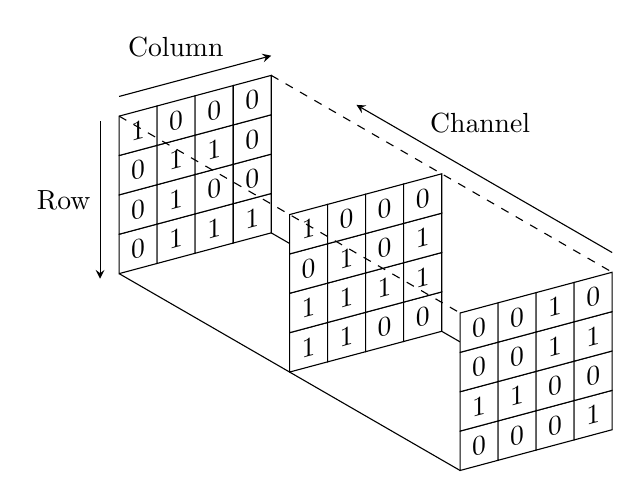
\begin{tikzpicture}[x=(15:.5cm), y=(90:.5cm), z=(330:.5cm), >=stealth]
    \draw (0, 0, 0) -- (0, 0, 10) (4, 0, 0) -- (4, 0, 10);
    \foreach \z in {0, 5, 10} \foreach \x in {0,...,3}
    \foreach \y [evaluate={\b=random(0, 1);}] in {0,...,3}
    \filldraw [fill=white] (\x, \y, \z) -- (\x+1, \y, \z) -- (\x+1, \y+1, \z) --
    (\x, \y+1, \z) -- cycle (\x+.5, \y+.5, \z) node [yslant=tan(15)] {\b};
    \draw [dashed] (0, 4, 0) -- (0, 4, 10) (4, 4, 0) -- (4, 4, 10);
    \draw [->] (0, 4.5, 0)  -- (4, 4.5, 0)   node [near end, above left] {Column};
    \draw [->] (-.5, 4, 0)  -- (-.5, 0, 0)   node [midway, left] {Row};
    \draw [->] (4, 4.5, 10) -- (4, 4.5, 2.5) node [near end, above right] {Channel};
  \end{tikzpicture}

\end{defbox}
\para{}
Ein Bild kann somit einfach als Tensor dritten Ranges $\ten{B} \in \set{R}^{h
  \times w \times c}$, der Form $(\text{Bildhoehe} \times \text{Bildbreite}
\times \text{Anzahl Farbkomponenten})$ betrachtet werden.
Elemente der Matrix nehmen dann einfach die Werte der Pixelkomponenten an.
Ein schwarzweiss Bild hat nur eine Komponente, welche die Helligkeit angibt.
Somit waere es eine normale 2D-Matrix $\mat{B} \in \set{R}^{h \times w}$ (siehe
Abb. (\ref{fig:bildmatrix})).
\para{}
\begin{figure}[h!]
  \begin{tikzpicture}

  \end{tikzpicture}
  \caption{Beispiel einer Bildmatrix}
  \label{fig:bildmatrix}
\end{figure}

\section{Topologie von CNNs}
Ein CNN besteht, wie ein KNN auch, aus Schichten. Jede dieser Schichten erhaelt
als Input ein Bild und hat auch wieder eines als Output. \\
Ein wichtiger Unterschied eines CNNs ist, dass es aus unterschiedlichen Typen von
Schichten besteht. Man unterscheiden zwischen drei Arten von Schichten:
\begin{itemize}
\item{\keyword{Fully-connected-Schichten},}
\item{\keyword{Convolutional-Schichten},}
\item{\keyword{Pooling-Schichten}, und}
\item{\keyword{Upsampling-Schichten}.}
\end{itemize}
Die fully-connected-Schicht ist altbekannt und ist einfach die klassische Schicht
eines KNNs, bestehend aus Neuronen. \\
Die Convolutional-Schicht ist eine neuartige Schicht, welche es im KNN nicht
gibt. Sie ist die Schicht, welche fuer das Training relevant ist,
da sie die Modellparameter beinhalten. Sie extrahiert die relevanten Features
aus den Inputbildern und lernt so die Bilder zu verstehen. \\
Die Pooling-Schicht, wie auch die Upsampling-Schicht beinhalten keine
Modellparameter und sind fuer das Training deshalb nicht direkt relevant.
Diese Schichten werden lediglich gebraucht um die verarbeiteten Bilder neu zu
skalieren. Dies ist sinnvoll, da durch die Extraktion gewisser Featurse, die
restlichen Features wegfallen. Somit muss weniger Information pro Bild gehalten
werden und die Bilder sollten schrumpfen um Overfitting vorzubeugen. Die Pooling-
Schichten reduzieren die Bilder und die Upsampling-Schichten erweitern die
Bilder um mehr Pixel. Dies wird in Sektion (\ref{sec:autoencoder}) fuer die Autoencoder
hilfreich werden. \\
Grundsaetzlich folgt auf eine Convolutional-Schicht immer entweder eine Pooling-
oder eine Upsampling-Schicht. Somit bilden sie gewissermassen eine Einheit.
\para{}
In Abbildung (\ref{fig:cnn_topology}) ist ein Schema eines CNNs abbgebildet.
\begin{figure}[h!]

  \caption{Schichtung eines CNNs}
  \label{fig:cnn_topology}
\end{figure}



\section{Convolutional-Schichten und Filter}
Zuerst betrachten wir die Convolutional Schicht. Diese Schicht macht ausgiebig
Gebrauch von sogennanten Filtern. Diese werden in diesem Abschnitt behandelt.

\subsection{Filter in der Bildverarbeitung}
\keyword{Filter} (auch Kerne) sind in der Bildverarbeitung sehr verbreitet. Jeder kennt sie entweder
von Photoshop, von Instagram oder sonstigen Bildbearbeitungsprogrammen.
Auch CNNs machen Gebrauch von solchen Filtern, in diesem Fall um die Features eines Bildes zu
erlernen.
\begin{figure}[h!]

  \caption{der Instagramfilter: Blablabla}
\end{figure}

\para{}
Ein Filter ist einfach eine Regionen, deutlich kleiner als das verarbeitete Bild
$\ten{B}$, welche
ueber alle Pixel wandert, diese manipuliert und so wieder ein neues Bild
$\tilde{\ten{B}}$ liefert.
Mathematisch gesehen handelt es sich bei einem Filter einfach um einen Tensor,
den sogennanten \keyword{Filtertensor} $\ten{F}$ oder Faltungstensor (siehe Abb.
(\ref{fig:filtermatrix})). Solche Filter sind immer quadratisch, wobei ihre
Zeilen- und Spaltenlaenge mit $f$ bezeichnet wird. Dabei ist $f$ immer eine ungerade Zahl, damit ein
Element, der sogennante \keyword{Zentralelement} (engl.: Center element), bezeichnet mit $(\ten{F})_C$,
immer im Zentrum des Filters liegt. \\

\begin{figure}[h!]
  % Sourcepixel kennzeichnen
  \caption{eine 2D-Filtermatrix}
  \label{fig:filtermatrix}
\end{figure}
\para{}
Das Verhalten des Filters wird durch seine Matrixeintraege bestimmt.
Die Elemente koennen also so gewaehlt werden, dass wenn der Filter auf ein Bild
angewandt wird, er bestimmte Features aus dem Bild hervorhebt. Solche Features
koennten zum Beispiel Raender oder Kanten sein, welche betont werden.
\para{}
Ein gutes Beispiel ist der Sobel-Filter. Er ist ein typischer 2D-Kantendetektions-Filter mit einer
Groesse von $f = 3$. Wir betrachten nun den Sobelfilter $\mat{G}_x$, welcher
horizontale Kanten akzentuiert. Die Eintraege dieses Filters lauten wie folgt:
\begin{equation*}
  \mat{G}_x =
  \begin{bmatrix}
    -1 & 0 & +1 \\
    -2 & 0 & +2 \\
    -1 & 0 & +1 \\
  \end{bmatrix}
\end{equation*}

Angewandt auf ein schwarz-weisses Bild $\mat{B}$, erhaelt man ein neues Bild, bei welchem alle erkannten
Katen weiss eingefaerbt sind und die restlichen Bereiche schwarz sind.
Der Filter erkennt dabei jede Stelle als Kante, welche zwei Regionen mit
genug grossem Kontrast voneinander trennt.
In Abbildung (\ref{fig:sobel_filter}) wurde der horizontale Sobelfilter auf ein
Beispielbild angewandt. Links ist das Ursprungsbild und rechts ist das
prozessierte Bild.


\begin{figure}[h!]

  \caption{Sobel-Filter angewandt auf Beispielsbild}
  \label{fig:sobel_filter}
\end{figure}

\para{}
\cite{wiki:sobel_operator}
\cite{deeplearning.ai:cnn}
\cite{wiki:kernel}


\subsection{Filter in CNNs}
Aus diktaktischen Gruenden betrachten wir nun zuerst
nur 2D-Filter, welche sich fuer graustufige Bilder
$\mat{B} \in \set{R}^{h \times w}$ eignen. Somit ist der hierfuer geeignete
Filter einfach eine 2D-Matrix, bezeichnet mit $\mat{F} \in \set{R}^{f \times
  f}$. Man bedenkte bei jeder Filtermatrix einfach immer, dass es sich
eigentlich im Allgemeinen Fall um einen 3D-Tensor handelt.
\para{}
Wie wir vorhin erfahren haben, koennen Filter genutzt werden um gewisse
Features eines Bildes hervorzuheben und andere Features zu ignorieren. Dabei
bestimmen die Filtereintraege, welche Features extrahiert werden. Somit bestimmt
die Aufgabe darin, die richtigen Filtereintraege zu bestimmen, damit die
gewuenschten Features erkannt werden und auf die gewuenschten Outputs abgebildet
werden. Naheliegend sollte jetzt der Gedanke sein, die Filtereintreage als die
Modellparameter eines CNNs zu definieren.
Mithilfe des Gradietenverfahrens sollten erneut diese Parameter
erlernt werden. \\
Da die Filter die gleiche Funktion haben, wie die Gewichte in einem KNN,
bezeichnet man die Filter in einem CNN mit $\ten{W}$. Die Groesse des Filters
stellt dabei einene Hyperparameter dar.

\begin{equation*}
  \mat{W} = \begin{pmatrix}
    w_{1,1} & \cdots & w_{1,f} \\
    \vdots & \ddots & \vdots \\
    w_{f,1} & \cdots & w_{f,f}
  \end{pmatrix}
\end{equation*}


\subsection{Filteroperation intutitiv}\label{sec:filteroperation_intuitiv}
Wie wendet man nun einen solchen Filter auf ein Bild an? Um das Prozedere einer
Filteroperation leichter verstaendlich zu machen, wird sie erneut fuer ein
graustufiges Bild $\mat{B} \in \set{R}^{h \times w}$ erlauetert. Spaeter werden auch noch farbige
Bilder erklaert.
\para{}
Bei einer Filteroperation, wendet man einen Filter $\ten{W}$ auf eine Bildtensor
$\ten{B}$ an und erhaelt so ein neues Bild $\tilde{\ten{B}}$. Man schreibt dafuer:
$\tilde{\ten{B}} = \ten{W} * \ten{B}$.
\para{}
Um nun diese Operation zu erklaeren, verwenden wir als Beispiel eine
2D-Filtermatrix $\mat{W} \in \set{R}^{3 \times 3}$, bei welcher
$f = 3$ gewaehlt wurde.
Wie bereits vorhin erwaehnt wandert der Filter ueber das Bild. Dabei befindet
sich der Filter immer ueber einer Region des Bilder, welche gleich gross ist,
wie der Filter selber (in diesem Fall ($3 \times 3$)), so dass den Filtermatrixeintraegen immer eindeutig
Bildmatrixeintraege entsprechen. Diese Region des Bildes bezeichnet man als das
\keyword{Rezeptive Feld} des Filters (siehe Abb. (\ref{fig:receptive_field})).
Das Zentralelement $(\ten{W})_c$ liegt dann gerade ueber dem sogennanten
\keyword{Quellenpixel} (engl.: source pixel), bezeichnet mit $(\ten{B})_S$.
Um das Rezeptive Feld zu kennzeichnen, bezeichnen wir es mit $\hat{\mat{B}}^{(y,x)}$, wobei die hochgestellten Indizes $(y,x)$ die Position
des Quellenpixel $(\mat{B})_S$ im Bild $\mat{B}$ angiebt. Somit ist das rezeptiven Feld einfach eine
Untermatrix $\tilde{\mat{B}} \in \set{R}^{3 \times 3}$ des Obermatrix $\mat{B}$.

\begin{figure}[h!]

  % Zentralelement einzeichnen mit Beschriftung
  \caption{ein Filter und sein rezeptives Feld}
  \label{fig:receptive_field}
\end{figure}

\para{}
Der Filter beginnt nun oben links ueber das Bild zu wandern. Somit
hat der Filter zu beginn das rezeptive Feld $\hat{\mat{B}}^{(2,2)}$, denn der
Filter darf nicht ueber die Raender des Bildes hinausragen.
Nun werden die Elemente der Filters mit den Elementen des rezeptiven Feldes
verrechnet, welche die gleichen Dimensionen besitzen. Dabei wird einfach das
Hadamard-Produkt (das elementweise Produkt) des beiden Matrizen miteinander
gebildet. Nun erhalten wir eine neue Matrix $\mat{W} \odot
\hat{\mat{B}}^{(2,2)} = \mat{P} \in \set{R}^{3 \times 3}$.
Nun werden noch alle Elemente der neuen Matrix $\mat{P}$
aufsummiert. Diese Zahl ist dann der Grauwert des ersten Pixels $(\tilde{\mat{B}})_{1,1}$ des bearbeiteten
Bildes (siehe Gl. (\ref{eq:filter1})). In diesem Sinne stellt der Filter eine Gewichtung der Nachbarspixel dar, welche
bestimmt, wie die neuen Pixel aussehen.
\\
\begin{equation}\label{eq:filter1}
  (\tilde{\mat{B}})_{1,1} = \sum_{y=1}^3 \sum_{x=1}^3 (\mat{P})_{y,x}
\end{equation}
\\
Nun wird der Filter um ein Element nach rechts verschoben und die gleiche
Prozedur angewendet, um den zweiten Pixel zu berechnen. Dies
wird durchgezogen, bis eine ganze Zeile der Bildmatrix durchstreift wurde.
Danach wird der Filter wieder nach ganz rechts verschoben und er bewegt sich ein
Element nach unten. Das geschieht, bis das ganze Bild verrechnet wurde.
Dabei werden die Elemente des urspruenglichen Bildes durchaus mehrmals
verrechnet, da es zu einer Ueberlappung des vorherigen Filter und des
verschobenen Filters kommt.
\para{}

\ifcp
\begin{figure}[h!]
  \centering
  % 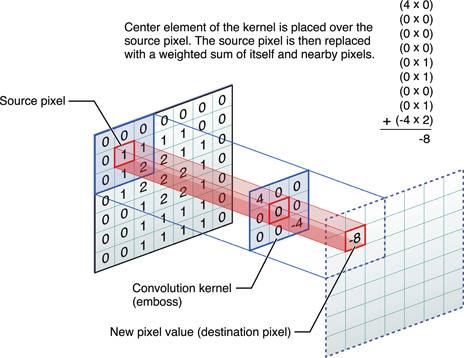
\includegraphics[width=0.5\textwidth]{conv.jpg}

  \makeatletter
  \tikzoption{canvas is xy plane at z}[]{%
    \def\tikz@plane@origin{\pgfpointxyz{0}{0}{#1}}%
    \def\tikz@plane@x{\pgfpointxyz{1}{0}{#1}}%
    \def\tikz@plane@y{\pgfpointxyz{0}{1}{#1}}%
    \tikz@canvas@is@plane
  }
  \makeatother

  \begin{tikzpicture}[x={(0.866cm,0.5cm)}, y={(-0.866cm,0.5cm)}, z={(0cm,1cm)}, scale=0.7,every pin/.style = {pin edge={Latex-,thin,black}}]


    \begin{scope}[canvas is xz plane at y=0,transform shape]
      % \draw[blue] (0,0) -- (10,0)--(10,10)--(0,10)--cycle;
      \foreach \ii [count = \xi] in {-3,-2,...,3}{
        \foreach \jj  [count = \yi] in {-3,-2,...,3}{
          \pgfmathsetmacro{\num}{int(abs(\ii)+abs(\jj))}
          \node[draw=blue!20!bgcolor,fill=blue!2!bgcolor,text=textcolor,minimum size=1cm] (n-1-\xi-\yi) at (\xi,-\yi) {\LARGE \num};
        }
      }
      \foreach \ii [count = \xi] in {-3,-2,-1}{
        \foreach \jj [count = \yi] in {-3,-2,-1}{
          \pgfmathsetmacro{\num}{int(abs(min(\ii,\jj))}
          \node[draw=blue!20!bgcolor,fill=blue!10!bgcolor,minimum size=1cm] (n-1-\xi-\yi) at (\xi,-\yi) {\LARGE \num}; % rename nodes
        }
      }

      \path[draw=textcolor] (n-1-1-1.north west) -- (n-1-7-1.north east) -- (n-1-7-7.south east) -- (n-1-1-7.south west) -- cycle;
      \path[draw=blue] (n-1-1-1.north west) -- (n-1-3-1.north east) -- (n-1-3-3.south east) -- (n-1-1-3.south west) -- cycle;


    \end{scope}

    \begin{scope}[canvas is xz plane at y=-7.3,transform shape]
      \foreach \ii [count = \xi] in {-1,0,1}{
        \foreach \jj  [count = \yi]in {-1,0,1}{
          \pgfmathsetmacro{\num}{int(\ii)}
          \node[draw=blue!20!bgcolor,fill=blue!10!bgcolor,text=textcolor,minimum size=1cm] (n-2-\xi-\yi) at (\xi,-\yi) {\LARGE \num};
        }
      }

      \path[draw=blue] (n-2-1-1.north west) -- (n-2-3-1.north east) -- (n-2-3-3.south east) -- (n-2-1-3.south west) -- cycle;
    \end{scope}

    \begin{scope}[canvas is xz plane at y=-11.2,transform shape]
      \foreach \ii [count = \xi] in {1,2,3,...,7}{
        \foreach \jj  [count = \yi]in {1,2,3,...,7}{
          \node[draw=blue!20!bgcolor,fill=blue!2!bgcolor,text=textcolor,minimum size=1cm] (n-3-\xi-\yi) at (\xi,-\yi) {};
        }
      }

      \foreach \ii [count = \xi] in {-3,-2,-1}{
        \foreach \jj [count = \yi] in {-3,-2,-1}{
          \pgfmathsetmacro{\num}{int(abs(min(\ii,\jj))}
          \node[draw=blue!20!bgcolor,fill=blue!10!bgcolor,minimum size=1cm] (n-3-\xi-\yi) at (\xi,-\yi) {}; % rename nodes
        }
      }

      \path[draw=blue,dashed] (n-3-1-1.north west) -- (n-3-3-1.north east) -- (n-3-3-3.south east) -- (n-3-1-3.south west) -- cycle;
      \path[draw=textcolor] (n-3-2-2.north west) -- (n-3-6-2.north east) -- (n-3-6-6.south east) -- (n-3-2-6.south west) -- cycle;
    \end{scope}

    % red box
    \path[draw=red,fill=red!50,opacity=0.3] (n-1-2-2.north east) -- (n-2-2-2.north east) -- (n-3-2-2.north east) -- (n-3-2-2.north west) -- (n-2-2-2.north west) -- (n-1-2-2.north west); % top
    \path[draw=red,fill=red!50,opacity=0.3] (n-1-2-2.south east) -- (n-2-2-2.south east) -- (n-3-2-2.south east) -- (n-3-2-2.south west) -- (n-2-2-2.south west) -- (n-1-2-2.south west); % bottom
    \path[draw=red,fill=red!50,opacity=0.3] (n-1-2-2.north east) -- (n-2-2-2.north east) -- (n-3-2-2.north east) -- (n-3-2-2.south east) -- (n-2-2-2.south east) -- (n-1-2-2.south east); % right
    \path[draw=red,fill=red!50,opacity=0.3] (n-1-2-2.north west) -- (n-2-2-2.north west) -- (n-3-2-2.north west) -- (n-3-2-2.south west) -- (n-2-2-2.south west) -- (n-1-2-2.south west); % left


    % blue lines connecting
    \path[draw=blue!40!bgcolor] (n-1-1-3.south west) -- (n-2-1-3.south west) -- (n-3-1-3.south west);
    \path[draw=blue!40!bgcolor] (n-1-3-1.north east) -- (n-2-3-1.north east) -- (n-3-3-1.north east);

    \node [pin=120:Rezeptives Feld $\hat{\mat{B}}^{(2,2)}$] at (n1-1-1.north west) {};
    \node [pin=180:Quellenpixel $(\mat{B})_S$] at (n1-2-2.east) {};
    \begin{scope}[canvas is xz plane at y=0,transform shape]
      \node[draw=red,minimum size=1cm] (marked1) at (2,-2) {\LARGE 2};
      % \node[] (sp-tag) at (n-1-2-2.north) {Quellenpixel $(\mat{B})_S$};
    \end{scope}

    \node [pin=180:Filter $\mat{F}$] at (n2-1-3.east) {};
    \begin{scope}[canvas is xz plane at y=-7.3,transform shape]
      \node[draw=red,text=textcolor,minimum size=1cm] (marked2) at (2,-2) {\LARGE 0};
      \node[] (rf-tag) at (n-2-2-1.north) {Filter $\mat{F}$};
      \node[] (ze-tag) at (n-2-2-2.north) {Zentralelement $(\mat{F})_C$};
    \end{scope}

    \begin{scope}[canvas is xz plane at y=-11.2,transform shape]
      \node[draw=red,fill=blue!10!white,text=textcolor,minimum size=1cm] (marked3) at (2,-2) {\LARGE -3};
    \end{scope}

  \end{tikzpicture}

  \caption{Schema, wie ein Filter ueber ein Bild laueft}
\end{figure}
\fi

Es ist zu bemerken, dass das neue Bild $\tilde{\mat{B}} \in \set{R}^{(h-2) \times (w-2)}$ nicht mehr die gleichen Masse
hat, wie das Ursprungsbild $\mat{B} \in \set{R}^{h \times w}$. Das liegt daran, dass pro
Lage des Filters jeweils nur ein Pixel des neuen Bildes berechnet wird. Man kann
sich vorstellen, dass an der Position des Quellenpixel jeweils ein neuer
Pixel entsteht. Dabei muss der Filter immer eine vollstaendige Region als
rezeptives Feld haben. Dadurch kommt das Zentralelement nie auf den Raendern des
Bilds zu liegen. Somit fallen diese weg.
\para{}
\cite{deeplearning.ai:cnn}
\cite{wiki:convolution}

\subsection{Filteroperationen als diskrete Faltungen}
Eigentlich handelt es sich bei einer Anwendung eines Filters auf ein Bild um
eine spezifische mathematische Operation: eine \keyword{diskrete Faltung} (engl.:
\keyword{Convolution}).
Daher ruehrt auch der Name des Convolutional Neural Networks.
Wir werden die Faltung als mathematische Operation nicht im vollen Umfang
betrachten, da sie relativ kompliziert ist. Wir werden uns lediglich auf die
Bedeutung der Faltung fuer Filter beschraenken.
Damit ihr die Defintion trotzdem mal gesehen habt:
\\
\begin{equation}
  (f * g)(x) = \int_{-\infty}^{\infty} f(\tau) g(x-\tau) \text{d}\tau
\end{equation}
\\
Streng genommen wird in CNNs nicht eine diskrete Faltung durchgefuehrt, sondern
eine sogennante \keyword{Kreuzkorrelation}. Der Unterschied dabei ist, dass bei einer
Kreuzkorrelation die Faltungsmatrix nicht zuerst horizontal, wie auch vertikal
gespiegelt wird, im Gegensatz zu der eigentlichen Faltung. Jedoch verwendet man
begrifflich das Wort Faltung fuer beide Operationen. Im Verlauf dieser Arbeit
wird mit dem Wort Faltung immer die Kreuzkorrelation gemeint sein.
\para{}
Mithilfe der Faltungsoperation koennen wir die Schritte welche in Sektion
(\ref{sec:filteroperation_intuitiv}) erklaert wurden zusammenfassen.
Bei der Filteroperation handlet es sich lediglich um eine diskrete Faltung des
Filtertensors $\ten{W}$ ueber den Bildtensor $\ten{B}$. Somit koennen wir
folgende Formel verwenden um einen Pixel $\tilde{\mat{B}}(x,y)$ des neuen Bildes zu berechnen.
\\
\begin{equation}
  \tilde{\mat{B}}_{y,x} = (\mat{W} * \mat{B})_{y,x} = \sum_{v=0}^{f-1} \sum_{u=0}^{f-1} \mat{W}_{v,u}\mat{B}_{y+v,x+u}
\end{equation}
\\
Fuer farbige Bilder ist das Vorgehen praktisch das selbe. Es werden nun
lediglich 3D-Tensoren anstatt 2D-Tensoren verwendet. Wir betrachten den
allgemeinen Bildtensor $\ten{B}_{h \times w \times c}$, wobei $c$ die Anzahl
Farbkomponenten (engl.: channels) ist.
Nun benutzt man einen Filter $\ten{W}_{f \times f \times c}$ mit beliebiger Groesse
$f$ aber mit der gleicher Tiefe $c$ wie das Ursprungsbild $\mat{B}$.
Dadruch muss der Filter nicht entlang der Tiefe des Bildes wandern, da er
gerade gleich tief ist, wie das Bild. Das hat zur Folge, dass das verarbeitete
Bild $\tilde{\mat{B}}$ immer eine 2D-Matrix ist.
Die allgemeine Filtergleichung lautet:
\\
\begin{equation}\tag{FO}
  \tilde{\mat{B}}_{y,x} = (\ten{W} * \ten{B})_{y,x} = \sum_{v=0}^{f-1} \sum_{u=0}^{f-1} \sum_{w=0}^c \ten{W}_{v,u,w} \ten{B}_{x+u,y+v,w}
\end{equation}

\subsection{Mehrere Filter}
Eine Filteroperation ist nicht auf einen einzigen Filter beschraenkt. Es koennen
mehrere Filter auf das gleiche Ausgangsbild angewandt werden und zusammen ein
Endbild erzeugen.
\para{}
Die Anzahl Filter bezeichnen wir mit $c$.
Nun macht man pro Filter $\ten{F}_i$ eine Faltung ueber das Ursprungsbild $\ten{B}$, wobei
jede Faltung einen neue Matrix $\tilde{\mat{B}}_i = \ten{F}_i * \ten{B}$ liefert, wobei $i$ der Index des
Filters ist. All diese gefalteten Bilder $\mat{B}*_i$ sind zweidimensionale Matrizen, unabhaengig davon, wieviel
Komponten das Ursprungsbild hatte. Aus diesem Grund koennen die einzelnen
Matrizen $\tilde{\mat{B}}_i$ aufeinander gelegt werden und somit einen grossen 3D-Endtensor
$\tilde{\ten{B}}$ bilden.
Hierfuer muessen alle Filter $\ten{F}_i$ gleich gross sein.
\begin{figure}[h!]
  \caption{aufeinander gelegte gefaltene Bilder}

\end{figure}
Die Tiefe des neuen Bildes $\tilde{\ten{B}}$ ist jetzt gerade die Anzahl Filter $c$.
Wir haben bereits frueher immer die Tiefe des Bildes (bzw. die Anzahl
Farbkomponenten) mit $c$ bezeichnet. Somit ist $c$ sowohl die Anzahl Filter
einer Schicht, wie auch die Tiefe des verarbeiteten Bildes.

\subsection{Padding}
Wie bereits erwaehnt schrumpfen die Bilder (an den Raendern), wenn man einen Filter auf sie anwendet.
Zur Erinnerung: Dies liegt daran, dass pro Lage des Zentralelement nur ein Pixel
des neuen Bildes entsteht und das Zentralelement nunmal nicht auf allen
Ursprungspixeln zu liegen kommt. Die Raender fallen so weg. Diese Groesse des
Wegfalls haengt von der Filtergroesse $f$ ab. Hierbei giltet folgende Formel fuer die
neue Groesse $n_1$ des Bildes, anhand der alten Groesse $n_0$.
\begin{equation}
  n_1 = n_0 - f + 1
\end{equation}

Das Problem hierbei ist, dass nach einigen Faltungen das Bild extrem geschrumpft
ist und im Grenzfall kleiner als der Filter wird. Das darf natuerlich nicht
passieren. Ausserdem kommt es dabei zu einem relativen Informationverlust an den Raender, da es im
Innern des Bildes zu viel Ueberlappungen der Filterlagen kommt und es bei den
Raendern nur seltener zur Ueberlappung kommt.
\para{}
Diese Probleme werden mit sogennantem \keyword{Padding} behoben. Padding ist ein
Schritt, welcher vor der eigentlichen Faltung stattfindet. Dabei werden einfach
zusatzliche Raender (Zeilen und Spalten) an das Ursprungsbild angebracht. Der
Tensor wird der Laenge und der Breite nach (nicht der Tiefe entlang!) an den Enden erweitert. Die neuen Elemente werden dabei auf den Wert
$0$ gesetzt.

\begin{figure}[h!]

  \caption{Padding}
\end{figure}

Das Padding $p$ ist eine Zahl, welche angibt wieviele Elemente an allen Raendern
hinzugefuegt werden. Padding $p = 1$ bedeutet, dass an allen Kanten jeweils eine
Reihe bzw. Spalte hinzugefuegt wird.
Begrifflich unterscheidet man zwei Arten von Padding:
\begin{itemize}
\item{\keyword{Valid-Padding}: Es werden keine zuesaezlichen Elemente angebracht. $f$ ist also 0.}
\item{\keyword{Same-Padding}: Es werden so viele Reihen und Spalten angebracht, dass
    die Groesse des Bildes nach der Faltung unveraendert bleibt.}
\end{itemize}
\para{}
Um Same-Padding durchzufuehren, muss man $p$ so waehlen, dass es den Wegfall durch
den Filter gerade kompensiert. Da durch das Padding das Bild der Laenge und
Breite nach jeweils um zwei $p$ laenger wird, erhaelt man den Ausdruck $n_1 =
n_0 - f + 1 + 2p$. Wenn man diese Formel jetzt nach $p$ aufloest,
erhaelt man folgende Formel fuer das Waehlen des Valid-Paddings $p$.
\\
\begin{equation}
  p = \frac{f-1}{2}
\end{equation}

\subsection{Stride}
Bis jetzt haben wir bei den Filterfaltungen, den Filter pro Anwendung immer nur
um einen Pixel verschoben. Das muss aber nicht so sein. Man kann den Filter
auch mit einer anderen Schrittgroesse verschieben. Diese Eigenschaft bezeichnet
man als \keyword{Stride} $s$. Falls $s = 2$ gewaehlt wird, bedeutet das, dass der
Filter sich pro Matrixmultiplikation um zwei Elemente bewegt. Somit wurde eine
Position uebersprungen. Zur Folge hat dies, dass das neue Bild
deutlich kleiner geworden ist, denn das Zentralelement uebspringt somit auch
diese Felder und bildet so deutlich weniger Pixel.
\para{}
Folgende Formel beschreibt die Dimensionen des neuen Bildes unter
beruecksichtigung der Filtergroesse $f$, dem Padding $p$ und dem Stride $s$.
\\
\begin{equation}
  n_1 = \frac{n_0 + 2p - f}{s} + 1
\end{equation}


\subsection{Vorzuege von Filtern}
Es stellt sich nun die Frage, weshalb sich Filter fuer Maschinelles
Lernen mit Bildern eignen.
Wie bereits erwaehnt besteht die Aufgabe von Filtern darin bestimmte Features
eines Bildes hervorzuheben und die restlichen auszublenden. Genau die gleiche
Aufgabe erfuellen die Neuronen in einem KNN. Auch sie sollen Features der
Inputsdaten erlernen, wobei gewisse Neuronen auf gewisse Features reagieren.
Weshalb verwendet man also nicht einfach KNNs? (abgesehen
von dem Problem mit der Ueberzahl an Modellparametern, siehe Sektion \ref{sec:CNN_parameter_problem}).
\para{}
Man muss erkennen, dass Bilddaten sich deutlich von sonstigen Daten unterscheiden.
Bildfeatures bzw. Pixel sind nur im Kontext von ihren Nachbarn relevant. Denn
ein Pixel ist erst dann eine Kante oder eine Ecke, wenn er zwei verschiedene
Farbregionen voneinander trennt. Oder ein Gegenstand wird erst durch eine ganzen Haufen
von Pixeln und deren relative Position zueinander ausgezeichnet.
Man bezeichnet diesen Umstand als \keyword{lokalisierte Features}.
\para{}
Desweiteren sind Bildausschnitte nicht immer gleich
orientiert. Wenn man ein Gesicht auf einem Bild erkennen moechte, sollte es aber
keine Rolle spielen, wo auf dem Bild es sich befindet, welche Groesse es
hat und was fuer eine Lage es hat. Um diese Eigenschaften irrelevant fuer das
Modell zu machen, muss dieses gewisse \keyword{Invarianzen} erfuellen.
\para{}
Die Eigenschaft, welche CNN geeignet macht fuer lokalisierte Features und
solche Invarianzen, bezeichnet man als \keyword{Parameter-Sharing}.
Sie bezeichnet den Umstand, dass auf
mehrere oder alle Features die gleichen Modellparameter wirken. Bei CNNs wird
dies durch die Bewegung der Filters bzw. seiner Eintraegen ueber (fast) alle
Pixel bewerkstelligt. Somit ist
es egal wo und wie sich die lokalisierten Features befinden. Dies fuehrt dann eben zu
den gewuenschten Invarianzen: Translations-, Rotations- und
Helligkeitsinvarianz. \\
Eine weiterer Vorteil durch dieses Parameter-Sharing ist, dass die Inputbilder
beliebige Dimensionen besitzen koennen, da die Filter ihre Bewegung lediglich an
die Groesse des Bildes anpassen muessen.

\subsection{die Convolutional-Schicht}
Nun moechten wir alles zusammentragen, was wir ueber Filter gelernt
haben, um nun die Convolutional-Schicht zu definieren.
\para{}
Beginnen tut eine Convolutional Schicht $l$ mit seinem Input, also den
Aktivierungen $\ten{A}^l \in \set{R}^{h^l \times w^l \times c^l}$, welche die vorherigen Schicht ($l-1$) produziert hat,
oder falls es die erste Schicht ist erhaelt sie den Input $\ten{X}$ des Netzes,
welchen man auch mit $\ten{A}^0$ bezeichnet. \\
Die Schicht besitzt $c^l$ Varianten an Filtern $\ten{W}^l_i \in
\set{R}^{f^l \times f^l \times c^{l-1}}$. Diese Filter haben alle die gleichen
Eigenschaften, bezueglich: der Groesse $f^l$, der Tiefe $c^{l-1}$, dem Padding
$p^l$, dem Stride $s^l$. Sie unterscheiden sich nur in den Modellparametern
$w^l_{i\,|\,\alpha,\beta,\gamma}$.
\\
\begin{equation*}
  \ten{W^l}_i =
  \begin{bmatrix}
    \begin{pmatrix}
      w_{i\,|\,1,1,1}^l & \cdots & w_{i\,|\,1,f,1}^l \\
      \vdots & \ddots & \vdots \\
      w_{i\,|\,f,1,1}^l & \cdots & w_{i\,|\,f,f,1}^l
    \end{pmatrix}
    & \stackrel{\mathclap{\normalfont\mbox{Tiefe}}}{\cdots} &
    \begin{pmatrix}
      w_{i\,|\,1,1,c^l}^l & \cdots & w_{i\,|\,1,f,c^l}^l \\
      \vdots & \ddots & \vdots \\
      w_{i\,|\,f,1,c^l}^l & \cdots & w_{i\,|\,f,f,c^l}^l
    \end{pmatrix}
  \end{bmatrix}
\end{equation*}
\\
Nun wendet faltet man jeden Filter $\ten{W}_i^l$ einzeln ueber das Bilder
$\ten{A}^l$ und erhaelt so mehrere neue 2D-Bilder $\tilde{\mat{A}}_i^l$.
\\
\begin{equation}
  \tilde{\mat{A}}_i^l = \ten{W}_i^l * \ten{A}^l
\end{equation}
\\
Die Faltung berechnet man nach folgender Gleichung:
\\
\begin{equation}\tag{FO}
  \tilde{\mat{A}}_{i\,|\,y,x}^l = (\ten{W}_i^l * \ten{A}^l)_{y,x} = \sum_{v=0}^{f-1} \sum_{u=0}^{f-1} \sum_{w=0}^c \ten{W}^l_{i\,|\,v,u,w} \ten{A}^l_{x+u,y+v,w}
\end{equation}
\\
Jede dieser Matrizen ist ein Querschnitt $\tilde{\mat{A}}^l_{:,:,i}$ entlang der
Tiefe des neuen 3D-Tensors $\tilde{\mat{A}}^l \in \set{R}^{h^{l+1} \times w^{l+1} \times c^l}$.
Hierbei ist die Tiefe $c^l$ gerade die Anzahl Filter $c^l$ und die Hoehe
$h^{l+1}$ und die Breite $w^{l+1}$ werden jeweils nach der folgenden Formel
berchnet anhand der Hohe $h^l$ und der Breite $w^l$ des Ausgangsbild.
\\
\begin{equation}
  n_1 = \frac{n_0 + 2p - f}{s} + 1
\end{equation}
\\
Da die Faltungsoperation eine lineare Operation, braucht man wieder eine
Aktivierungsfunktion, um das Modell zu befaehigen nicht-lineare Probleme zu
loesen.
Deshalb wendet man in einem letzten Schritt die vektorisierte Aktivierungsfunktion
$\vecf{\varphi}$ auf den Tensor $\tilde{\mat{A}}^l$ an und erhaelt so die
neue Aktiverung der naechsten Schicht $\ten{A}^{l+1}$. Meistens waehlt man hier
die ReLU-Aktiverungsfunktion $\vecf{\varphi}^{ReLU}$.
\begin{equation}
  \ten{A}^{l+1} = \vecf{\varphi}(\tilde{\ten{A}}^l)
\end{equation}



\cite{Goodfellow-et-al-2016}

\section{Dimensionalitaetskontrolle}
Beim Anwenden einer Convolutional Schicht gehen Informationen verloren, da nur
die relevanten Features hervorgehoben werden und der Rest verworfen wird. Jedoch
schrumpft das Bild entweder gar nicht (bei Same-Padding) oder es schrumpft nur
sehr leicht (bei Valid-Padding). Dies ist ein Problem, da die Information in
deutlich weniger Pixeln bzw. Tensorelementen codiert werden koennte. Deshalb
haben wir einen unoetigen Ressourcenverbrauch und eine erhoehte Gefahr fuer
Overfitting. Um diesem Problem entgegenzuwirken gibt es einerseits sogennante
\keyword{Pooling-Schichten} und als Gegenstueck dazu
\keyword{Upsampling-Schichten}. Ersteres wird verwendet um die Dimensionalitaet
der Bilder zu vermindern und letzteres um die Dimensionalitaet der Bilder zu
erweitern. Somit ermoeglich diese Schichten eine kontrollierte Art (im Gegensatz zum
Padding) die Dimensionalitaet einzustellen.

\subsection{die Pooling-Schicht}
Die Pooling-Schicht verringert die Dimensionalitaet durch das Zusammenfassen eines Felds
von Tensorelementen zu einem einzigen Tensorelement der naechsten Schicht
erreicht. Dabei geht das Feld nur entlang der Laenge und Breite des Bildes und
nicht entlang der Tiefe. Dies bedeutet, das Pooling wird auf jeden Channel
einzeln angewandt, dadurch aendert sich die Tiefe des Bildes nicht.
\para{}
Fuer die Beschreibung einer Pooling-Schicht wird viel Begrifflichkeit der
Convolutional-Schicht und der Filter uebernommen.
Die Groesse des Elementfelder, welches zusammengefasst wird, bezeichent man analog zur
Filtergroesse mit $f^l$. Das Stride $s^l$ bezeichnet auch beim Pooling wieder wie
gross dieSchrittgreosse beim Verschieben des Felder ist. Meistens waehlt man den
Stride $s$ gerade gleich der Feldgroesse $f$, damit alle Pixel
zusammengefasst werden. Kleiner als $f$ kann $s$ nicht gewaehlt werden.
\para{}
Man unterscheidet zwischen zwei Arten von Pooling:
\begin{itemize}
  \item{\keyword{Average-Pooling}: Das Elementenfeld wird zusammengefasst, indem
    man das arithmetische Mittel der Element bildet.}
  \item{\keyword{Max-Pooling}: Das Elementenfeld wird zusammengefasst, indem das
    Element mit dem hoehsten Wert beibehalten wird und die anderen verworfen werden.}
\end{itemize}
In Praxis verwendet man eigentlich nur Max-Pooling, da es deutlich bessere
Resultate erziehlt.
\para{}
Es ist festzustellen, dass eine Pooling-Schicht keinerlei Modellparameter
besitzt. Somit gibt es nichts zu trainieren. Sie besitzt lediglich einige
Hyperparameter, wie die Feldgroesse $f$ und den Stride $s$.
\para{}
Mit einer Pooling-Schicht, bei welcher $f = 2$ und $s = 2$ gewaehlt wurde, also
ein ($2 \times 2$)-Feld zusammengefasst wird, kommt es zu einer
Dimensionalitaetsreduktion von 75\%, da aus jeweils vier Element ein Element wird.
\para{}
Um zu berechnen, was die neuen Dimensionen nach dem Pooling sind, gelten sie
gleichen Formeln wie fuer die Filteroperationen:
\\
\begin{equation}
  n_1 = \frac{n_0 - f}{s} + 1
\end{equation}
\\

\subsection{die Upsampling-Schicht}
Die Upsampling-Schicht bildet das Gegenstueck zur Pooling-Schicht, da sie die
Dimensionaliaet der Bilder erhoeht. Auf den ersten Blick erscheint unklar,
weshalb man die Dimensionalitaet erhoehen wollen koennte, da die eigentliche
Motivation dieser Schichten in der Verhinderung von Overfitting besteht. Jedoch
sollte in Kapitel (\ref{sec:autoencoder}) klar werden, weshalb solche Schicht
noetig sind.
\para{}
Man verwendet auch hier wieder den Begriff der Feldgroesse $f^l$. Diesemal
beschreibt dieser Wert, wie stark das Bild hochskaliert wird. Beim Upsampling
wird ein Element zu einem $(f \times f)$-Feld hochgerechnet und erweitert so die
Dimensionalitaet.
\para{}
Es stellt sich natuerlich die Frage, was fuer Werte das neue Feld erhaelt.
Dafuer muss man eine Interpolationsart waehlen.
Zwei Arten sind besonders verbreitet:
\begin{itemize}
\item{\keyword{Bilineare Interpolation}}
\item{\keyword{Naechste-Nachbar-Interpolation} (engl.: nearest-neighbor-interpolation)}
\end{itemize}
Wir werden hier nur die Naechste-Nachbar-Interpolation betrachten. Sie ist
ziemlich trivial, denn alle neuen Feldelemente nehmen einfach den Wert des alten
Elements an. Der Wert wird also einfach vermehrt.

\pagebreak
\chapter{Autoencoder}\label{sec:autoencoder}
Ein \keyword{Autoencoder} ist eine weitere KNN-Architektur eines KNNs. Diese
Architekur beschreibt jedoch nicht die Schichtenarten, sondern beschreibt das
Netzwerk auf der Ebene der Netzform. Autoencoder werden verwendet um \keyword{effiziente
Daten-Codierungen} zu erlernen. Dies bedeutet das Modell versucht die
wichtigsten Features, welche die meisten Informationen codieren zu extrahieren
und diese in einer neuer Form zu repraesentieren. Er kann dann aus dieser neuen
Form dann wieder eine der Ursprungsform sehr aehnliche Repraesentation reproduzieren.
\para{}

benutzt um effiziente Codierungen von Daten zu erlernen. Strenggenommen gehoert
er dem unueberwachtem Lernen bei, da die Daten keine Labels beinhalten. Jedoch
ist diese Begrifflichkeit etwas irrefuehrend, da der Autoencoder trotzdem darauf
trainiert wird, gewisse gewuenschte Outputs zu liefern. Die Labels sind naemlich
in diesem Fall einfach gerade die Inputs.
Semi-unueberwacht deshalb, weil die Labels in den Features enthalten sind.

Der Autoencoder soll eine komprimierte Repraesentation (Encoding) fuer einen
Datensatz erlernen und somit die wesentlichen Features herausextrahieren. Er
kann so zur \keyword{Dimensionalitaetsreduktion} verwendet werden. Dabei faellt
das ``Rauschen''(engl.:Noise) der Daten weg. Das Netzwerk rekonstruiert dann
anhand der Codierung wieder die urspruenglichen Daten.



\section{Topologie von Autoencodern}

\begin{itemize}
\item{Eingabeschicht}
\item{Flaschenhals/Encoding}
\item{Ausgabeschicht/Decoding}
\end{itemize}

\begin{figure}[h!]
  \centering
  \begin{tikzpicture}[>=latex]

    \tikzstyle{netstyle} = [matrix of nodes,nodes={draw,circle,inner sep=0, minimum size=1cm},column sep=0.5cm,row sep=-9pt]
    \tikzstyle{cl} = [draw=none,fill=none]
    \tikzstyle{heading} = [clear,text width=15mm,text centered]
    \tikzstyle{inp} = [fill=red!70!bgcolor]
    \tikzstyle{hid} = [fill=blue!70!bgcolor]
    \tikzstyle{ou} = [fill=green!70!bgcolor]

    \matrix[netstyle] (mat)
    {
      |[inp]| $x_1$  & |[cl]| & |[cl]| & |[cl]| & |[cl]| & |[cl]| & |[ou]|$\tilde{x}_1$ \\
      |[cl]| & |[hid]|$h_1^1$   & |[cl]| & |[cl]| & |[cl]| & |[hid]|$h_1^3$  & |[cl]|  \\
      |[inp]| $x_2$  & |[cl]| & |[hid]|$h_2^2$ & |[cl]| & |[hid]| $h_2^4$ & |[cl]| & |[ou]|$\tilde{x}_2$ \\
      |[cl]| & |[hid]|$h_2^1$   & |[cl]| & |[hid]| $h_2^3$ & |[cl]| & |[hid]|$h_2^3$ & |[cl]| \\
      |[inp]| $x_3$ & |[cl]| & |[hid]|$h_3^2$ & |[cl]| & |[hid]| $h_3^4$ & |[cl]| & |[ou]|$\tilde{x}_3$ \\
      |[cl]| & |[hid]|$h_3^1$   & |[cl]| & |[cl]| & |[cl]| & |[hid]|$h_3^3$ & |[cl]| \\
      |[inp]| $x_4$ & |[cl]| & |[cl]| & |[cl]| & |[cl]| & |[cl]| & |[ou]|$\tilde{x}_4$ \\
    };

    % titels
    \node [yshift=1cm] (text) at (mat-1-4) {Flaschenhals};
    \path [draw,ultra thick,->,>=stealth] (text) -- ($(text)!0.7!(mat-3-4)$);

    % dots
    % \node [yshift=-1cm,scale=2] at (mat-7-1) {$\vdots$}; % for inputs
    % \node [yshift=-1cm,scale=2] at (mat-6-3) {$\vdots$};
    % \node [yshift=-1cm,scale=2] at (mat-7-4) {$\vdots$};
    % \node [yshift=-1cm,scale=2] at (mat-6-5) {$\vdots$};
    % \node [yshift=-1cm,scale=2] at (mat-7-7) {$\vdots$}; % for outputs

    % input -> hidden1
    \foreach \ai in {1,3,...,7} {
      \foreach \aii in {2,4,6}
      \draw[->] (mat-\ai-1) -- (mat-\aii-2);
    }

    % hidden1 -> hidden2
    \foreach \ai in {2,4,...,6} {
      \foreach \aii in {3,5}
      \draw[->] (mat-\ai-2) -- (mat-\aii-3);
    }

    % hidden2 -> hidden3
    \foreach \ai in {3,5} {
      \foreach \aii in {4}
      \draw[->] (mat-\ai-3) -- (mat-\aii-4);
    }

    % hidden3 -> output
    \foreach \ai in {4} {
      \foreach \aii in {3,5}
      \draw[->] (mat-\ai-4) -- (mat-\aii-5);
    }

    % hidden3 -> output
    \foreach \ai in {3,5} {
      \foreach \aii in {2,4,6}
      \draw[->] (mat-\ai-5) -- (mat-\aii-6);
    }

    % hidden3 -> output
    \foreach \ai in {2,4,6} {
      \foreach \aii in {1,3,...,7}
      \draw[->] (mat-\ai-6) -- (mat-\aii-7);
    }

  \end{tikzpicture}
  \label{fi:nn_layers}
  \caption{Schichten eines Autoencoders}
\end{figure}

\section{Mathematische Betrachtung}
Falls lineare Neuronen verwendet werden, ist der Prozess der
Dimensionalitaetsreduktion sehr aehnlich zur Hauptkomponentenanalyse.

Mathematik:


\begin{gather}
  \phi: \mathcal{X} \to \mathcal{F}\\
  \psi: \mathcal{F} \to \mathcal{X}\\
  \ds\phi,\psi = \operatorname*{\arg \min}_{\phi,\psi} \norm{X - (\phi \circ \psi)X}^2
\end{gather}

\section{Bedeutung von Autoencodern}
\subsection{Datenkompression}
Falls ein Autoencoder nur aus linearen Neuronen besteht, ist die
Dimensionsreduktion sehr aehnlich zu der Hauptkomponentenanalyse.

Problem: Netzwerk versucht Durchschnitt aller Trainingsdaten zu erlernen.
\subsection{Datengenerierung}
\subsection{Eigenschaften erkennen}

\section{Convolutional-Autoencoder}

\section{Denoising-Autoencoder}


% ------------------------------------

\chapter{Entwicklung eines Denoising-Autoencoders}
In diesem Kapitel moechten wir uns nun der eigentlichen Entwicklung eines
Machine-Learning-Modells widmen. Wir werden zuerst einige Frameworks und Tools,
welche diese Entwicklung ermoeglichen betrachten und ihre grobe Funktionsweise
verstehen. In einem naechsten Schritt programmieren wir dann ein konkretes Modell.

\section{TensorFlow}
\keyword{TensorFlow}, kurz TF, ist ein von Google entwickeltes Framework fuer
datenstromorientriere Programmierung. Es ist im Grunde genommen ein
Mathematik-Framework, dessen Hauptanwendungsbereich im Maschinellen Lernen liegt.
TF ist in C++ und Python geschrieben. Das
Python-Frontend ermoeglicht ein sehr einfaches erstellen von Computation Graphs
um Modelle fuer Maschinelles Lernen zu designen.
TF ist gratis und ein Open-Source-Projekt. Es kann auf Github gefunden werden
unter: https://github.com/tensorflow/tensorflow.


\subsection{Hardwarebeschleuniging}
TF ist hauptsaechlich in C++ geschrieben, da diese Programmiersprache sehr
nah am Maschinen Code ist (engl.: low-level), im Gegensatz zu vielen anderen Programmiersprachen.
Somit ist der Code sehr hardwarenah und kann sehr schnell ausgefuehrt werden.
\para{}
\keyword{Hardwarebeschleuniging} (engl. Hardware Acceleration)

\keyword{Parallelisierung}

\subsubsection{CPU-Beschleunigung}

\subsubsection{GPU-Beschleunigung und CUDA}

\subsection{Funktionsweise}

\subsubsection{Tensoren}

\subsubsection{Computation Graphs}

\subsection{Tensorboard}

\section{Keras}
\keyword{Keras} ist ein Open-Source Deep-Learning Framework geschrieben in
Python. Keras wurde entwickelt um eine einheitliche Schnittstelle fuer
verschieden Backends, wie TensorFlow, Microsoft Cognitive Toolkit und Theano zu
bieten. Seit TF Version 1.4 ist Keras ein fester Bestandteil der TensorFlow-Core-API.

Keras ermoeglicht ein sehr simples und benutzerfreundliches defnieren von
Deep-Learning-Modeln welche dann sehr einfach trainiert werden koennen.

\section{Setup}
Installationsschritte fuer Python, CUDA, CUDNN und Tensorflow auf arch-basierter Linuxdistribution mit Pacman.

Emacs und Spacemacs erwaehnen.

\section{das Modell}
Denoising Autoencoder fuer den MNIST-Datensatz.

\subsection{MNIST}

\section{Entwicklung}


\chapter{Diskussion}


%%% Local Variables:
%%% mode: latex
%%% TeX-master: "../main"
%%% End:
